% NeurIPS 2026 Submission
% IMPORTANT: Download neurips_2026.sty from https://neurips.cc/Conferences/2026/CallForPapers
% and place it in the same directory as this file.
%
% Compile with: pdflatex main.tex && bibtex main && pdflatex main.tex && pdflatex main.tex
%
% Switch options:
%   \usepackage{neurips_2026}            % anonymous submission (use this for submission)
%   \usepackage[preprint]{neurips_2026}  % preprint (shows author info)
%   \usepackage[final]{neurips_2026}     % camera-ready

\documentclass{article}

\usepackage{neurips_2026}   % anonymous/blind review mode

\usepackage[utf8]{inputenc}
\usepackage[T1]{fontenc}
\usepackage{hyperref}
\usepackage{url}
\usepackage{booktabs}
\usepackage{amsfonts}
\usepackage{nicefrac}
\usepackage{microtype}
\usepackage{xcolor}
\usepackage{amsmath}
\usepackage{amssymb}
\usepackage{graphicx}
\usepackage{subcaption}
\usepackage{multirow}
\usepackage{wrapfig}
\usepackage{enumitem}

\graphicspath{{../inputs/figures/}}

% ---------------------------------------------------------------
\title{From EEG to Image: Decoding Visual Mental Imagery\\
via Language-Mediated Generation and Direct CLIP Alignment}
% ---------------------------------------------------------------

% Anonymous for blind review -- remove for camera-ready
\author{%
  Anonymous Author(s)\\
  % Uncomment below for camera-ready:
  % Manoj Kumar Tiwari \\
  % School of Artificial Intelligence and Data Science (SAIDE)\\
  % Indian Institute of Technology Jodhpur\\
  % \texttt{manojtiwari1.2v@gmail.com}
}

\begin{document}
\maketitle

% ===============================================================
\begin{abstract}
% ===============================================================
When a person closes their eyes and imagines an object, their brain generates electrical activity that partially reflects the imagined object's visual properties. If we could decode these brain signals and render them as images, we would open a direct channel from thought to visual output---a capability with profound implications for assistive communication, brain-computer interfaces, and our scientific understanding of mental imagery. In this work, we address the problem of translating raw electroencephalography (EEG) signals, recorded while subjects \emph{imagine} visual objects, into photorealistic images of those objects. We design and compare two complete end-to-end pipelines evaluated on a 10-class cross-subject benchmark using the Figshare Visual Imagery EEG dataset (22 subjects). Both pipelines use a frozen CSBrain foundation model as a shared EEG feature extractor and an anatomy-aware token reduction module. \textbf{Pipeline~2 (EEG-LLM)} routes EEG features through a language model: a projection network maps EEG representations into TinyLlama-1.1B's embedding space, LoRA fine-tuning teaches the language model to generate class-descriptive text from brain signals, and Stable Diffusion~2.1 synthesises the final image. \textbf{Pipeline~3 (EEG-CLIP)} eliminates the language step entirely: a compact 4.8M-parameter EEGCLIPMapper---a Q-Former-style transformer network---directly aligns EEG features with CLIP's visual embedding space and conditions Stable Diffusion~v1.5. Both pipelines substantially exceed the 10\% chance baseline. Pipeline~3 achieves \textbf{35.8\%} test accuracy versus 32.6\% for Pipeline~2, at a fraction of the computational cost (4.8M vs.\ $\sim$1.2B effective parameters). A key finding is that CLIP \emph{image} embeddings of stimulus photographs (mean pairwise cosine similarity $\approx$0.54) are far more discriminative contrastive training targets than CLIP \emph{text} embeddings of class names ($\approx$0.90), explaining why direct visual alignment outperforms language-mediated decoding.
\end{abstract}

% ===============================================================
\section{Introduction}
% ===============================================================

\subsection{The Problem: Reading Visual Thought}

When you imagine a dog, your brain does not merely retrieve a verbal label or an abstract concept---it constructs an internal visual representation that activates many of the same neural circuits involved in \emph{actually seeing} a dog~\citep{kosslyn2001neural}. This process, called visual mental imagery, produces measurable electrical activity in the brain that carries, at least partially, information about the imagined object's category. The ability to decode this activity and render it as a visible image would mean that a person could communicate visual intent or mental content without any motor action---purely through thought.

This capability is not merely an academic curiosity. For individuals who have lost the ability to speak or move---due to conditions such as amyotrophic lateral sclerosis (ALS), locked-in syndrome, or severe cerebral palsy---brain-computer interfaces (BCIs) represent one of the few remaining channels of communication with the outside world. Current BCIs largely focus on spelling text through imagined motor commands or eye movements~\citep{birbaumer2000bci}. An imagery-to-image BCI, by contrast, could allow such individuals to express visual concepts, communicate needs, or create---without relying on any residual motor function. Understanding how mental imagery is represented in brain signals is therefore both a fundamental scientific question and a practical engineering problem with direct humanitarian relevance.

\subsection{Why EEG?}

Brain signals can be recorded by several modalities. Functional magnetic resonance imaging (fMRI) measures changes in blood oxygenation and provides high spatial resolution (millimetre scale), allowing researchers to identify which brain regions activate during a task. However, fMRI is expensive (thousands of dollars per hour), requires the subject to lie motionless inside a large magnetic scanner, has poor temporal resolution (1--2 seconds per measurement), and is completely impractical for everyday BCI use.

Electroencephalography (EEG) works on a fundamentally different principle: metal electrodes placed on the scalp measure the tiny electrical potentials generated by the synchronised firing of large populations of cortical neurons. EEG offers millisecond temporal resolution, captures dynamic temporal patterns in brain activity (alpha waves, gamma bursts, event-related potentials), is non-invasive and safe, requires only a wearable headset, and is comparatively inexpensive. These properties make EEG uniquely suited for practical BCI applications.

The trade-off is signal quality. EEG suffers from several sources of noise: muscle activity (especially from jaw and eye movements), environmental electrical interference, volume conduction (signals from a localised brain region spread and are detected by many electrodes simultaneously), and inherent inter-subject variability in skull thickness and brain anatomy. As a result, EEG signals carrying mental imagery information are considerably weaker and noisier than fMRI signals. Achieving high-quality image reconstruction from EEG is therefore a substantially harder problem than from fMRI.

\subsection{The Core Challenge: Mental Imagery Under Cross-Subject Conditions}

Most prior deep learning work on brain-to-image reconstruction has focused on \emph{visual perception}---reconstructing what a subject is currently looking at---rather than \emph{visual imagery}---reconstructing what a subject is currently imagining~\citep{ozcelik2023brain,scotti2024mindeye}. Perception and imagery recruit overlapping but distinct neural circuits, and critically, perceptual EEG contains much stronger stimulus-locked responses (signals that consistently peak at the same latency after the stimulus onset). Imagery EEG lacks this strong temporal anchor, making it inherently harder to decode.

A second, equally important challenge is \emph{cross-subject generalisation}. EEG signals are highly individual: two people imagining the same object produce qualitatively different spatial patterns of activity due to anatomical differences, cognitive style differences, and varying levels of imagery vividness. A model that learns subject-specific features during training will simply not work on a new person. For any real-world BCI application, the system must be able to generalise to users it has never seen before---a property we call \emph{zero-shot cross-subject generalisation}. This is the setting we evaluate in this paper.

\subsection{What Has Been Tried Before}

Early approaches to EEG-based image generation used class-conditional generative adversarial networks (GANs). ThoughtViz~\citep{tirupattur2018thoughtviz} and Brain2Image~\citep{kavasidis2017brain2image} trained GAN generators conditioned on EEG class embeddings, producing blurry but semantically relevant images across a handful of categories. These methods used subject-dependent training and were not evaluated cross-subject. More importantly, GAN-based generation at that time could not produce photorealistic images. The advent of large-scale generative models changed this. Stable Diffusion~\citep{rombach2022ldm}, a latent diffusion model trained on billions of image-text pairs, can produce photorealistic images from text or CLIP~\citep{radford2021clip} embedding conditioning. Bai et al.~\citep{bai2023brain} combined EEG encoding with CLIP-guided Stable Diffusion and demonstrated that CLIP alignment substantially improves both classification accuracy and image quality---providing the most direct precedent for our work.

On the fMRI side, Ozcelik \& VanRullen~\citep{ozcelik2023brain} and MindEye~\citep{scotti2024mindeye} showed that mapping fMRI features to CLIP space and conditioning a diffusion model can reconstruct perceived images at impressive quality. While these methods are not directly applicable to EEG (different modality, different SNR regime, different spatial resolution), they establish the general principle that aligning brain signals to CLIP space is a viable and powerful strategy.

A parallel line of work has developed self-supervised \emph{foundation models} for EEG---models pre-trained on large, diverse EEG corpora that learn transferable representations applicable to many downstream tasks~\citep{kostas2022bendr,jiang2024labram,zhu2024csbrain}. These models, analogous to BERT or GPT in natural language processing, provide a strong starting point for downstream EEG decoding without requiring task-specific feature engineering.

\textbf{The gap.} Despite this progress, two questions remain unanswered: (1) Is it better to route EEG features through language (EEG $\to$ text $\to$ image) or to align directly to visual embedding space (EEG $\to$ CLIP $\to$ image) for mental imagery decoding? (2) When training the CLIP alignment, should we use CLIP image embeddings of the stimulus photographs or CLIP text embeddings of class names as training targets? These questions have not been systematically studied for visual imagery EEG under cross-subject conditions.

\subsection{Our Approach and Findings}

We design, train, and compare two end-to-end EEG-to-image pipelines that answer these questions head-on.

\textbf{Pipeline~2 (EEG-LLM)}\footnote{We label our systems Pipeline~2 and Pipeline~3 to maintain consistency with our broader experimental framework, in which Pipeline~1---a simple linear probe (logistic regression on mean-pooled CSBrain features) that achieved 18.3\% test accuracy---served as an early cross-subject sanity check confirming that CSBrain features carry class-discriminative information. Pipeline~1 is not described in detail as it involves no novel components; we include it here only to clarify the numbering convention.} routes through language. EEG features are projected into a large language model's embedding space, the model (TinyLlama-1.1B, fine-tuned with LoRA) generates a class-descriptive text prompt, and Stable Diffusion~2.1 synthesises the final image from that text.

\textbf{Pipeline~3 (EEG-CLIP)} bypasses language entirely. We introduce the \textbf{EEGCLIPMapper}, a compact Q-Former-inspired transformer network that maps EEG features directly to CLIP's visual embedding space. The predicted CLIP embedding directly conditions Stable Diffusion~v1.5. We train the mapper with a carefully designed composite loss that simultaneously promotes class discriminability, contrastive alignment with CLIP image prototypes, and sequence-level alignment with CLIP text representations.

Our key findings are: (1) Pipeline~3 achieves 35.8\% test accuracy versus 32.6\% for Pipeline~2---direct CLIP alignment outperforms language mediation. (2) The EEGCLIPMapper does this with 4.8M parameters versus $\sim$1.2B for Pipeline~2 and trains $\sim$10$\times$ faster. (3) The reason direct alignment wins is quantifiable: CLIP image embeddings of the 10 stimulus classes have mean pairwise cosine similarity 0.54 (the classes are well-separated in this space), while CLIP text embeddings have mean pairwise similarity 0.90 (nearly indistinguishable). Text targets provide almost no useful training signal for contrastive learning.

\textbf{Contributions:}
\begin{enumerate}[noitemsep,topsep=2pt]
  \item Two complete, reproducible EEG-to-image pipelines on the Figshare 10-class cross-subject benchmark, including all preprocessing, training, and evaluation code.
  \item The \textbf{EEGCLIPMapper}: a 4.8M-parameter Q-Former-style network that bridges 20 EEG region tokens to the 77-token, 768-dimensional CLIP conditioning format required by Stable Diffusion.
  \item An empirical and geometric explanation of why CLIP image embeddings (pairwise sim $\approx$0.54) are far superior contrastive targets to CLIP text embeddings ($\approx$0.90) for EEG alignment.
  \item A two-phase training strategy that prevents conflicting gradient directions from the MSE and cosine alignment objectives, yielding 2--4\% accuracy gains applicable to general multimodal CLIP-alignment problems.
\end{enumerate}

% ===============================================================
\section{Related Work}
% ===============================================================

\textbf{EEG decoding and foundation models.}
EEG decoding---classifying cognitive states or imagined stimuli from raw electrode recordings---has been studied for decades. Classical methods relied on hand-crafted spectral features such as event-related synchronisation/desynchronisation and Common Spatial Patterns (CSP)~\citep{blankertz2007bci}, which require domain expertise to design and are fragile across sessions and subjects. Deep learning changed this substantially: EEGNet~\citep{lawhern2018eegnet} introduced a compact depthwise-separable CNN that generalised well across BCI paradigms, and EEG-Conformer~\citep{song2023eegconformer} combined CNNs with self-attention to capture both local spectrotemporal and global sequential patterns. However, these methods still train from scratch on small datasets, limiting their representational power. The most recent generation of self-supervised EEG foundation models---BENDR~\citep{kostas2022bendr}, LaBraM~\citep{jiang2024labram}, and CSBrain~\citep{zhu2024csbrain}---adopt the BERT-style masked pre-training paradigm on large multi-subject, multi-dataset corpora. By pre-training on diverse EEG signals, these models learn spatiotemporal representations that transfer broadly to downstream tasks without task-specific feature engineering, in the same way that GPT-based language models transfer to many NLP tasks.

\textbf{Brain-to-image reconstruction.}
The idea that visual brain activity encodes categorical and low-level image properties was established by seminal neuroscience work~\citep{haxby2001distributed,kay2008identifying}. Early deep learning approaches to image reconstruction used GANs: Shen et al.~\citep{shen2019end} reconstructed perceived images from fMRI using a multi-stage GAN, while ThoughtViz~\citep{tirupattur2018thoughtviz} and Brain2Image~\citep{kavasidis2017brain2image} extended the paradigm to EEG. These early EEG methods produced semantically rough images and required subject-specific models. The field advanced sharply when latent diffusion models~\citep{rombach2022ldm} provided a powerful generative backbone conditioned on CLIP embeddings. Ozcelik \& VanRullen~\citep{ozcelik2023brain} and MindEye~\citep{scotti2024mindeye} demonstrated that mapping fMRI features to CLIP space enables high-quality image reconstruction of \emph{perceived} scenes. For EEG specifically, Bai et al.~\citep{bai2023brain} showed that CLIP-guided diffusion substantially improves both classification and generation quality over prior GAN-based approaches---a finding that directly motivates our Pipeline~3 design. Our work extends this line by (a) operating in the harder mental imagery (not perception) setting, (b) evaluating under strict cross-subject conditions, (c) introducing the EEGCLIPMapper architecture for a more principled EEG-to-CLIP alignment, and (d) providing the first systematic comparison of language-mediated versus direct CLIP alignment strategies.

\textbf{Cross-modal alignment and Q-Former architectures.}
CLIP~\citep{radford2021clip} is a vision-language model trained on 400 million image-text pairs using contrastive learning. It learns a shared embedding space in which matching images and text are close, and it has become the dominant conditioning interface for text-to-image generation. Aligning a new modality (EEG, fMRI, audio) to CLIP space has emerged as the standard strategy for leveraging pre-trained generative models. The challenge is that EEG naturally produces a variable-length sequence of electrode-patch tokens, while CLIP conditioning requires a fixed-format embedding. The Q-Former mechanism from BLIP-2~\citep{li2023blip2} and the Perceiver Resampler from Flamingo~\citep{alayrac2022flamingo} solve this by maintaining a fixed number of learnable query embeddings that attend (via cross-attention) to the variable-length input, producing a fixed-length output in the target embedding space. Our EEGCLIPMapper directly adapts this design to bridge 20 EEG region tokens to the 77-token CLIP conditioning format.

% ===============================================================
\section{Dataset and Data Preparation}
% ===============================================================

\subsection{Study Design and Data Collection}

The data used in this work comes from the \textbf{Figshare Visual Imagery EEG dataset}~\citep{figshare_eeg} (DOI: 10.6084/m9.figshare.30227503), a publicly available benchmark specifically designed for EEG-based visual imagery decoding. Understanding exactly how this data was collected is essential for appreciating what the decoding task requires and why it is difficult.

\textbf{Subjects.} Twenty-two healthy adult volunteers participated in the study. All subjects had normal or corrected-to-normal vision and reported no history of neurological disorders. EEG was recorded using the standard international 10--20 electrode placement system with 32 channels arranged on the scalp, covering the full head from prefrontal to occipital regions. The 32 electrodes were sampled at 1,000 Hz, meaning 1,000 voltage readings per second per channel, resulting in a data rate of 32,000 measurements per second per subject.

\textbf{Stimulus protocol.} Each trial followed a two-stage paradigm designed to capture \emph{mental imagery} rather than passive visual perception. In the first stage (perception), a colour photograph of one of the 10 target objects was displayed on a screen for approximately 2 seconds while the subject viewed it naturally. In the second stage (imagery), the screen went blank, the subject closed their eyes, and was instructed to \emph{mentally visualise the object they just saw as vividly as possible for 4 seconds}. The EEG signal recorded during this 4-second closed-eyes imagery period is what we use in our experiments. We do \emph{not} use the perception-stage EEG because our goal is to decode mental imagery, not visual perception---the signals during eyes-closed imagery are weaker, noisier, and more variable, but they are what a real BCI would need to work with.

\textbf{Stimulus classes.} The 10 classes span three semantic domains to provide a range of visual complexity: \textbf{Animals}---Dog, Bird, Fish; \textbf{Geometric Figures}---Pentagram, Square, Circle; \textbf{Everyday Objects}---Scissors, Watch, Cup, Chair. Each subject completed multiple trials per class, yielding approximately 350--400 trials per subject across all classes, for a total of roughly 8,000 trials in the full dataset. A complete class-label mapping is given in Appendix~\ref{app:class_mapping}.

\subsection{Featurisation: Which Part of the EEG Signal We Use}

A raw trial, as delivered by the EEG amplifier, is a matrix of size $32 \; (\text{channels}) \times 4000 \; (\text{time samples at 1000 Hz})$ representing the 4-second mental imagery window. However, we do \emph{not} pass this raw high-rate signal directly into our models. Instead, we apply a sequence of domain-standard preprocessing steps that reduce noise, remove artefacts, and reshape the signal into the format expected by the CSBrain foundation model. The preprocessed and reshaped representation---not the raw signal---is what enters the feature extraction stage.

\subsection{Preprocessing Pipeline}

We process each raw trial through the following steps in order:

\textbf{Step 1 --- Channel selection and ordering.} We retain all 32 channels arranged according to the standard 10--20 montage. The channel ordering is standardised across all subjects to ensure consistency, since different recording setups may label channels in different orders.

\textbf{Step 2 --- Unit conversion and baseline correction.} EEG amplifiers output signals in raw amplifier units (arbitrary integers). We convert these to microvolts ($\mu$V) using the dataset-provided calibration factors. We then apply channel-wise baseline correction: for each channel, we subtract the mean voltage computed over a 200\,ms pre-imagery baseline window (just before the imagery period begins). This removes slow drifts and DC offsets that vary across sessions and subjects.

\textbf{Step 3 --- Bandpass filtering.} We apply a 5th-order Butterworth bandpass filter with cutoff frequencies 0.3--50\,Hz (zero-phase, applied forwards and backwards to avoid phase distortion). This serves two purposes. The high-pass cutoff at 0.3\,Hz removes slow baseline drifts and breathing-related artefacts. The low-pass cutoff at 50\,Hz removes electrical line noise (50\,Hz mains interference, common in Indian and European labs) and high-frequency muscle artefacts (EMG) that contaminate scalp EEG. The frequency range 0.3--50\,Hz contains the neurophysiologically meaningful EEG bands: delta (1--4\,Hz), theta (4--8\,Hz), alpha (8--13\,Hz), beta (13--30\,Hz), and low gamma (30--50\,Hz).

\textbf{Step 4 --- Trial extraction.} Using the event markers recorded in the EEG file (indicating the onset of each imagery period), we extract a 4-second window from 0\,ms to 4000\,ms relative to imagery onset for each trial, yielding a segment of size $32 \times 4000$.

\textbf{Step 5 --- Downsampling.} We downsample from 1,000\,Hz to 200\,Hz by keeping every 5th time point, reducing the temporal dimension from 4,000 to 800 samples per channel. This is safe because the bandpass filter already removed all content above 50\,Hz; by the Nyquist theorem, a 200\,Hz sampling rate can faithfully represent signals up to 100\,Hz, well above our 50\,Hz cutoff. Downsampling reduces the input size by 5$\times$ and makes the model computationally tractable without losing any meaningful neural information.

\textbf{Step 6 --- Patch reshaping.} Following CSBrain's input convention, we reshape the $32 \times 800$ matrix into $32 \times 4 \times 200$---that is, 32 channels each divided into 4 consecutive temporal patches of 200 samples (1 second each). This produces 128 electrode-patch tokens, each of dimension 200, which is the raw input format for CSBrain.

\textbf{Step 7 --- Amplitude normalisation.} We divide all values by 100\,$\mu$V, a typical peak amplitude for EEG signals. This ensures that model inputs are in approximately the $[-1, 1]$ range, facilitating stable gradient flow during training.

\subsection{Dataset Split}

A strict subject-based split is used throughout all experiments. Subjects 1--16 form the \textbf{training set} ($\sim$5,000--6,000 trials). Subjects 17--19 form the \textbf{validation set} ($\sim$1,000--1,200 trials). Subjects 20--22 form the \textbf{test set} ($\sim$1,000--1,200 trials). Crucially, \emph{no trial from any test or validation subject appears during training}, and model selection (choosing the best checkpoint) is done solely based on validation accuracy. This strict cross-subject protocol ensures that all reported results measure generalisation to completely unseen individuals---the condition required for real-world deployment. Trial-level splitting (randomly mixing trials from all subjects) would allow the model to simply memorise subject-specific patterns, massively inflating apparent accuracy; we deliberately avoid this.

% ===============================================================
\section{Method}
% ===============================================================

\subsection{Problem Formulation}

We frame the problem formally as follows. We observe a collection of EEG trials $\{(\mathbf{x}_i, y_i)\}_{i=1}^{N}$, where each $\mathbf{x}_i \in \mathbb{R}^{32 \times 800}$ is the preprocessed EEG signal recorded while subject $i$ mentally imagined an object, and $y_i \in \{0, 1, \ldots, 9\}$ is the corresponding class label indicating which of 10 objects was imagined. Our goal is to train a mapping $f: \mathbb{R}^{32 \times 800} \to \mathcal{I}$ that takes a raw EEG trial as input and produces a photorealistic image $\hat{I} \in \mathcal{I}$ that correctly depicts the imagined object. We decompose this mapping into two stages: an \emph{EEG decoding} stage that predicts the imagined class or produces a conditioning embedding, followed by an \emph{image synthesis} stage that renders the prediction as a photorealistic image. We fix the image synthesis stage (Stable Diffusion) and focus our training effort entirely on the EEG decoding stage.

\subsection{Shared Frontend: CSBrain Encoder and EEGTokenReducer}

\textbf{CSBrain encoder.}
Both pipelines begin with the same frozen feature extractor: the CSBrain foundation model~\citep{zhu2024csbrain}. CSBrain is a transformer-based EEG encoder pre-trained using masked signal modelling on a large multi-subject, multi-task EEG corpus. During pre-training, random patches of the input EEG are masked and the model learns to reconstruct them from the remaining context---analogous to masked language modelling in BERT. This forces the model to learn deep spatiotemporal representations that capture the statistical structure of brain activity across many subjects and cognitive tasks.

The CSBrain encoder $f_\mathrm{enc}: \mathbb{R}^{C \times P \times S} \to \mathbb{R}^{C \times P \times D}$ takes the reshaped input ($C=32$ channels, $P=4$ temporal patches, $S=200$ samples per patch) and processes it through a series of modules: (i) a Conv2D temporal patch embedding that captures spectral content via a real FFT projection, (ii) learnable depthwise-separable Conv2D positional encoding that tells the model which electrode and which time patch each token corresponds to, (iii) 1D convolutional temporal embedding with multi-scale kernels $\{1, 3, 5\}$ to capture patterns at different temporal scales, (iv) a brain-region interaction module that models correlations between anatomically related electrode groups, and (v) a 12-layer cross-regional transformer encoder whose self-attention operates across the full set of electrode-patch tokens. The output is $\mathbf{H} = f_\mathrm{enc}(\mathbf{X}) \in \mathbb{R}^{C \times P \times D}$ with $D = 200$ features per token. We \emph{freeze} all CSBrain weights throughout training---they are never updated. This is a deliberate design choice: since our training set contains only $\sim$6,000 trials from 16 subjects, fine-tuning a 12-layer transformer would risk catastrophic overfitting to subject-specific patterns. By keeping CSBrain frozen, all trainable parameters in our system are concentrated in the much smaller downstream components, which must learn to read and re-map the foundation model's features without modifying the foundation model itself.

\textbf{EEGTokenReducer.}
CSBrain produces $C \times P = 32 \times 4 = 128$ electrode-patch tokens. While this fine-grained representation is rich, directly processing 128 tokens downstream would be computationally expensive and would not naturally reflect the hierarchical organisation of the brain. We therefore introduce an anatomy-aware token reduction step. Specifically, we group the 32 electrodes into five anatomical brain regions based on the standard 10--20 electrode map (see Appendix~\ref{app:channels} for the complete grouping): Frontal (8 channels, covering forehead and prefrontal cortex), Fronto-central (5 channels, covering motor planning areas), Central (5 channels, covering primary motor and somatosensory cortex), Parietal (9 channels, covering association areas involved in spatial attention and imagery), and Occipital (5 channels, covering primary visual cortex). Within each region, we average the CSBrain output tokens across the constituent electrodes:
\begin{equation}
  \hat{\mathbf{H}}_r = \frac{1}{|\mathcal{E}_r|} \sum_{c \in \mathcal{E}_r} \mathbf{H}_{c,:,:} \in \mathbb{R}^{P \times D},
  \quad \hat{\mathbf{H}} \in \mathbb{R}^{5 \times P \times D} = \mathbb{R}^{20 \times 200}.
\end{equation}
This reduces 128 tokens to $5 \times 4 = 20$ region-patch tokens while preserving both temporal structure (4 time patches) and spatial structure (5 brain regions). The reduction is parameter-free and requires no training; it relies entirely on known neuroanatomy. The resulting 20-token sequence $\hat{\mathbf{H}} \in \mathbb{R}^{20 \times 200}$ is the shared input to both pipelines.

\begin{figure}[htbp]
  \centering
  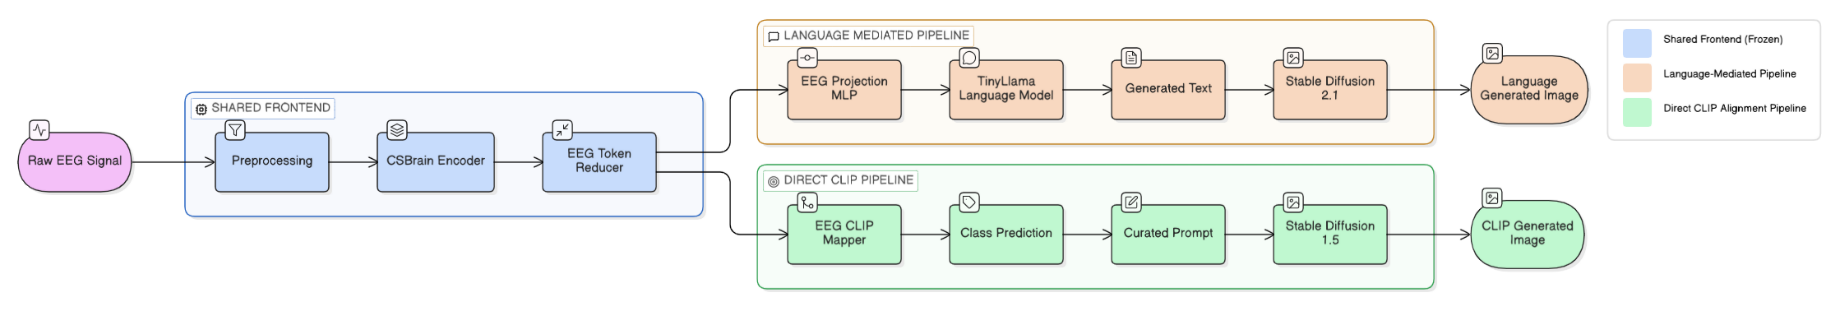
\includegraphics[width=\linewidth]{architecture.png}
  \caption{System architecture. Both pipelines share a frozen CSBrain encoder and EEGTokenReducer frontend (grey). Pipeline~2 (orange) routes through TinyLlama-1.1B with LoRA to produce a class-descriptive text that drives Stable Diffusion~2.1. Pipeline~3 (green) maps EEG tokens directly to CLIP space via EEGCLIPMapper, conditioning Stable Diffusion~v1.5.}
  \label{fig:architecture}
\end{figure}

\subsection{Pipeline 2: Language-Mediated Generation (EEG-LLM)}

The intuition behind Pipeline~2 is that modern text-to-image models (Stable Diffusion) are highly capable when given a good natural language description. If we can teach a language model to generate such a description from EEG features, we can leverage Stable Diffusion's full generative power without training an image generator from scratch. The challenge is bridging the gap between the 200-dimensional EEG feature space and the 2048-dimensional embedding space of TinyLlama-1.1B~\citep{zhang2024tinyllama}.

\textbf{Projection MLP.} We train a two-layer MLP $g: \mathbb{R}^{20 \times 200} \to \mathbb{R}^{20 \times 2048}$ that maps each of the 20 EEG tokens to TinyLlama's embedding dimension:
\[
g(\hat{\mathbf{H}}) = \text{Linear}(2048 \to 2048) \circ \text{Dropout}(0.1) \circ \text{GELU} \circ \text{Linear}(200 \to 2048).
\]
The projected 20 EEG tokens are prepended to TinyLlama's input token sequence, acting as a soft prompt that conditions the language model on the subject's brain state.

\textbf{Efficient LLM fine-tuning.} TinyLlama-1.1B is a 1.1-billion-parameter causal language model. Training or even fully fine-tuning it would require substantial VRAM and compute. We use two complementary techniques to make this tractable on consumer hardware. First, we load TinyLlama in 4-bit NF4 quantisation using BitsAndBytes, which compresses the model's weights from 32-bit floats to 4-bit integers, reducing its VRAM footprint from $\sim$2.2\,GB to $\sim$0.7\,GB with minimal accuracy loss. Second, we apply LoRA (Low-Rank Adaptation)~\citep{hu2022lora}: instead of updating all 1.1B weights, we insert small trainable low-rank matrices ($r=8$, $\alpha=16$) into the query and value projection layers of every attention block, yielding only $\sim$1.2M additional trainable parameters. The frozen quantised weights provide the language model's general capabilities, while the LoRA matrices learn to adapt its output to the EEG-conditioned text generation task.

\textbf{Training objective.} We train the projection MLP and LoRA parameters jointly using the standard causal language modelling (next-token prediction) loss:
\begin{equation}
  \mathcal{L}_\mathrm{LM} = -\sum_{l=1}^{L} \log P_\theta(t_l \mid \mathbf{e}_\mathrm{EEG}, t_1, \ldots, t_{l-1}),
\end{equation}
where $t_1, \ldots, t_L$ is the target class-descriptive text (e.g., ``An image of a dog. The animal has four legs and fur.'') and $\mathbf{e}_\mathrm{EEG}$ are the projected EEG embeddings prepended to the sequence. The model learns to predict each word of the target description given the EEG context and the preceding words.

\textbf{Inference.} At test time, the EEG from a new subject is passed through the frozen CSBrain encoder and EEGTokenReducer, projected by the MLP, and fed to TinyLlama to generate a text description (greedy decoding). This text is then passed directly to Stable Diffusion~2.1 (DPMSolver++ scheduler, 25 denoising steps, guidance scale 7.5) to synthesise the final 512$\times$512 image.

\subsection{Pipeline 3: Direct CLIP Alignment via EEGCLIPMapper (EEG-CLIP)}

Pipeline~3 takes a fundamentally different route. Rather than generating text as an intermediate representation, we ask: can we train a network to directly predict, from EEG features, the CLIP embedding that Stable Diffusion uses as its conditioning signal? If so, we cut out the language step entirely and condition the diffusion model directly on a predicted visual embedding derived from brain activity.

The challenge is architectural: CLIP image embeddings for Stable Diffusion conditioning have a specific format---a sequence of 77 tokens each of dimension 768, plus a single pooled 768-dimensional vector---while our EEG features are a sequence of 20 tokens each of dimension 200. We design the EEGCLIPMapper to perform this mapping through four stages:

\textbf{Stage 1 --- Input projection.} Each of the 20 EEG region-patch tokens is passed through a small MLP:
\[
\text{LayerNorm} \to \text{Linear}(200 \to 512) \to \text{GELU} \to \text{Dropout}(0.1) \to \text{Linear}(512 \to 512),
\]
lifting each token from dimension 200 to dimension 512, which is the mapper's internal working dimension.

\textbf{Stage 2 --- Transformer encoder.} The 20 projected tokens are passed through a 4-layer pre-norm transformer encoder (8 attention heads, internal dimension 512, feedforward dimension 1024, dropout 0.1). This self-attention stage allows the mapper to model dependencies between different brain regions and time windows---for example, correlations between occipital (visual) and frontal (attention) tokens that may collectively indicate which object is being imagined.

\textbf{Stage 3 --- Q-Former expansion.} We maintain a set of $M=77$ learnable query embeddings $\mathbf{Q} \in \mathbb{R}^{77 \times 512}$, initialised randomly and updated during training. These queries attend to the 20 EEG tokens as keys and values via cross-attention:
\[
\text{output} = \text{Attention}(\mathbf{Q},\; \mathbf{z}^{(4)},\; \mathbf{z}^{(4)}) + \mathbf{Q},
\]
where $\mathbf{z}^{(4)}$ are the transformer outputs and the residual connection ensures gradient flow during early training. The 77 queries ``attend to'' the 20 EEG tokens and each learns to extract a different aspect of the EEG representation. The output is a 77-token sequence of dimension 512---expanded from the 20 EEG tokens to match CLIP's token count.

\textbf{Stage 4 --- Output projection.} The 77 tokens are projected from dimension 512 to dimension 768 via LayerNorm followed by a linear layer, producing the sequence output $\mathbf{Z}^{\text{seq}} \in \mathbb{R}^{77 \times 768}$. In parallel, the sequence is mean-pooled and passed through a Tanh-activated linear layer to produce the pooled embedding $\bar{\mathbf{z}} \in \mathbb{R}^{768}$. Tanh bounds outputs to $[-1, 1]$, matching the typical range of normalised CLIP embeddings and preventing gradient explosion during early training.

Total trainable parameters in EEGCLIPMapper: $\sim$4.8M.

\textbf{Loss function and training targets.} We train the EEGCLIPMapper with a composite loss that simultaneously drives four complementary objectives:
\begin{equation}
  \mathcal{L} = \lambda_\mathrm{cls}\,\mathcal{L}_\mathrm{cls} + \lambda_\mathrm{cont}\,\mathcal{L}_\mathrm{cont} + \lambda_\mathrm{cos}\,\mathcal{L}_\mathrm{cos} + \lambda_\mathrm{mse}\,\mathcal{L}_\mathrm{mse},
\end{equation}
with weights $(\lambda_\mathrm{cls}, \lambda_\mathrm{cont}, \lambda_\mathrm{cos}, \lambda_\mathrm{mse}) = (5.0, 2.0, 1.0, 0.1)$.

The \textbf{classification loss} $\mathcal{L}_\mathrm{cls}$ is a standard cross-entropy loss applied via a linear classification head on top of the pooled EEG embedding $\bar{\mathbf{z}}$:
\[
\mathcal{L}_\mathrm{cls} = -\sum_{k=0}^{9} \mathbb{1}[y=k]\,\log\,\sigma(\mathbf{W}_\mathrm{cls}\,\bar{\mathbf{z}})_k.
\]
This directly optimises for correct class prediction and is the most direct training signal available.

The \textbf{InfoNCE contrastive loss} $\mathcal{L}_\mathrm{cont}$ pulls the EEG embedding toward the CLIP image embedding of the correct class prototype and pushes it away from the other nine:
\[
\mathcal{L}_\mathrm{cont} = -\log\frac{\exp(\bar{\mathbf{z}}^\top\mathbf{v}_y / \tau)}{\sum_{k=0}^{9} \exp(\bar{\mathbf{z}}^\top\mathbf{v}_k / \tau)},
\]
with temperature $\tau=0.5$. Here $\{\mathbf{v}_k\}_{k=0}^{9}$ are the 10 CLIP image class prototype vectors, computed by passing the 10 stimulus photographs through the frozen CLIP ViT-L/14 image encoder and taking their mean per class. These are fixed 768-dimensional vectors that serve as targets throughout training.

The \textbf{cosine alignment loss} $\mathcal{L}_\mathrm{cos}$ directly maximises the cosine similarity between the EEG embedding and the target CLIP image prototype:
\[
\mathcal{L}_\mathrm{cos} = 1 - \frac{\bar{\mathbf{z}} \cdot \mathbf{v}_y}{\|\bar{\mathbf{z}}\|\,\|\mathbf{v}_y\|}.
\]
This complements the contrastive loss by providing a differentiable absolute alignment signal independent of the other classes.

The \textbf{MSE sequence alignment loss} $\mathcal{L}_\mathrm{mse}$ aligns the full 77-token sequence output to the hidden states produced by the CLIP text encoder for the corresponding class-name prompt (e.g., ``a photo of a dog''):
\[
\mathcal{L}_\mathrm{mse} = \frac{1}{77}\sum_{l=1}^{77}\|\mathbf{Z}^{\text{seq}}_l - \mathbf{t}_y^{(l)}\|_2^2,
\]
where $\mathbf{t}_y \in \mathbb{R}^{77 \times 768}$ are the CLIP text encoder hidden states for class $y$, obtained from the aMUSEd-512 model's text encoder. Importantly, \emph{the sequence output $\mathbf{Z}^{\text{seq}}$ conditions Stable Diffusion's cross-attention layers}, which were pre-trained to receive CLIP text encoder tokens as keys and values. Aligning our sequence output to CLIP text hidden states (rather than image embeddings) therefore ensures format-compatibility with the diffusion model's cross-attention interface, while the pooled-embedding losses ($\mathcal{L}_\mathrm{cont}$, $\mathcal{L}_\mathrm{cos}$) handle the semantic alignment to CLIP image space. We chose the aMUSEd-512 text encoder specifically because it is a fine-tuned CLIP text encoder whose output format is matched to Stable Diffusion v1.5's cross-attention dimensions ($77 \times 768$), avoiding a dimension mismatch that arises with the standard ViT-L/14 text encoder ($77 \times 768$ but with different normalisation conventions). The two-phase training schedule (Section~\ref{sec:training}) is essential to prevent this MSE term from destabilising the image-space alignment established during warmup.

\textbf{Why image embeddings and not text embeddings as primary targets?}
A central empirical finding of this work is that using CLIP \emph{image} embeddings as the targets for $\mathcal{L}_\mathrm{cont}$ and $\mathcal{L}_\mathrm{cos}$ dramatically outperforms using CLIP \emph{text} embeddings. The reason is geometric: the 10 CLIP image class prototype embeddings have a mean pairwise cosine similarity of approximately 0.54, meaning different object classes are well-separated in CLIP image space and the contrastive loss receives meaningful gradients that distinguish between classes. The 10 CLIP text embeddings of class-name prompts (``a photo of a dog'', ``a photo of a bird'', etc.) have a mean pairwise cosine similarity of approximately 0.90, meaning they are nearly indistinguishable in CLIP text space. When text embeddings are used as targets, the InfoNCE denominator is dominated by near-equal terms for all classes, and the gradient signal for moving the EEG embedding toward the correct class versus away from incorrect classes is essentially zero. We analyse this in detail in Section~\ref{sec:analysis}.

\subsection{Two-Phase Training Strategy}
\label{sec:training}

Training all four loss terms simultaneously from a random initialisation leads to suboptimal convergence. The root cause is a geometric conflict: $\mathcal{L}_\mathrm{mse}$ pulls the mapper's output toward the CLIP \emph{text} embedding space, while $\mathcal{L}_\mathrm{cos}$ and $\mathcal{L}_\mathrm{cont}$ pull it toward the CLIP \emph{image} embedding space. These two subspaces are not aligned in the 768-dimensional CLIP embedding space, so during early training when the mapper is largely uninitialised, these conflicting gradients prevent either objective from making progress.

We resolve this with a two-phase schedule:

\textbf{Warmup phase (epochs 1--5):} Only $\mathcal{L}_\mathrm{cls}$, $\mathcal{L}_\mathrm{cont}$, and $\mathcal{L}_\mathrm{cos}$ are active ($\mathcal{L}_\mathrm{mse}$ is disabled). The learning rate is $5 \times 10^{-4}$. During these epochs, the mapper learns to produce embeddings that are discriminative and approximately aligned with CLIP image space---establishing a stable geometric structure without interference from the sequence-level MSE objective.

\textbf{Joint phase (epochs 6--20):} All four losses are active. The learning rate drops to $10^{-4}$ and decays with cosine annealing to $10^{-6}$ over the remaining epochs. Gradient clipping at norm 1.0 prevents instability from outlier batches. By this point, the mapper already produces reasonable image-space embeddings; the MSE term can now refine the sequence output format without destabilising the learned embedding geometry.

For Pipeline~2, an analogous warmup is applied: the projection MLP is trained at $5\times$ the base learning rate during the warmup phase to ensure EEG-to-LLM alignment is established before LoRA begins modifying the language model's attention patterns.

% ===============================================================
\section{Experiments}
\label{sec:experiments}
% ===============================================================

\subsection{Research Questions}

Our experiments are designed to answer three concrete questions:
(1) Can either pipeline decode the imagined class from EEG at above-chance accuracy under strict cross-subject evaluation?
(2) Does direct CLIP alignment (Pipeline~3) outperform language-mediated generation (Pipeline~2), and if so, why?
(3) What visual categories are easier or harder to decode, and does this pattern align with neuroscientific expectations?

\subsection{Experimental Setup}

All experiments were run on a single consumer-grade GPU with 6--8\,GB VRAM (Intel Core i7, 16\,GB DDR4 RAM, Windows~11). This is deliberately a low-resource setting to demonstrate that meaningful EEG-to-image decoding does not require large-scale compute infrastructure. Both pipelines were trained for 20 epochs total (5 warmup + 15 joint), with effective batch size 32 achieved via gradient accumulation over 8 micro-batches of size 4. We used the AdamW optimiser with weight decay 0.01 and cosine annealing learning rate schedule. Image synthesis used DPMSolver++ at 25 denoising steps, guidance scale 7.5, $512 \times 512$ resolution, and fixed random seed 42 for reproducibility. All code was written in PyTorch~$\geq$2.0 with mixed-precision float16 training and HuggingFace Transformers and Diffusers libraries. Complete hyperparameter tables are provided in Appendix~\ref{app:hyperparams}.

\subsection{EEG Decoding Accuracy}

Table~\ref{tab:accuracy} reports the classification results on the held-out test set (subjects 20--22, never seen during training or model selection). The most important baseline is 10\%---the accuracy a model would achieve by randomly guessing among 10 equally likely classes. Both pipelines substantially exceed this baseline, confirming our first research question: EEG signals recorded during visual imagery carry class-discriminative information that persists across subjects and can be extracted by a trained model.

\begin{table}[h]
  \centering
  \caption{Test set EEG decoding accuracy (10 classes, chance = 10\%).}
  \label{tab:accuracy}
  \begin{tabular}{lccc}
    \toprule
    \textbf{Metric} & \textbf{Chance} & \textbf{Pipeline~2 (EEG-LLM)} & \textbf{Pipeline~3 (EEG-CLIP)} \\
    \midrule
    Top-1 classifier accuracy      & 10.0\% & 32.6\%  & \textbf{35.8\%} \\
    Keyword match accuracy         & --     & 35.1\%  & -- \\
    Nearest-neighbour (CLIP space) & --     & --      & 29.4\% \\
    Best validation accuracy       & --     & 36.2\%  & 38.4\% \\
    Trainable parameters           & --     & $\sim$1.2B & \textbf{4.8M} \\
    Training time / epoch          & --     & 2--3\,h & 15--25\,min \\
    \bottomrule
  \end{tabular}
\end{table}

Pipeline~3 outperforms Pipeline~2 by 3.2 percentage points (35.8\% vs.\ 32.6\%) while using over 250$\times$ fewer trainable parameters and training approximately 10$\times$ faster per epoch. This answers our second research question: direct CLIP alignment is both more accurate and more efficient than language-mediated generation.

The keyword matching accuracy for Pipeline~2 (35.1\%) slightly exceeds its top-1 classifier accuracy (32.6\%). This discrepancy arises because the LLM occasionally places the correct keyword in an incorrect context (e.g., generating ``imagining a chair with a dog sitting on it''), which the keyword heuristic counts as a correct prediction while the classifier correctly identifies the mismatch. For Pipeline~3, the gap between classifier accuracy (35.8\%) and nearest-neighbour accuracy in CLIP space (29.4\%) indicates that the linear classification head has learned more effective decision boundaries than raw cosine similarity in the high-dimensional CLIP space---a common phenomenon when the decision boundary is not well-approximated by a hyperplane through the origin.

\subsection{Contextual Comparison with Prior EEG Decoding Methods}
\label{sec:prior_comparison}

No published work has been evaluated on the Figshare Visual Imagery EEG dataset (released 2024), making direct numerical comparison impossible. We therefore provide a contextual comparison in Table~\ref{tab:sota} situating our results within the broader EEG visual decoding literature. Two factors make direct comparison non-trivial: (1) most prior EEG methods operate on visual \emph{perception} (subjects viewing images) rather than visual \emph{imagery} (subjects imagining images)---the latter is substantially harder due to the absence of stimulus-locked EEG responses; (2) prior work uses different datasets, subject counts, and class sets.

\begin{table}[h]
  \centering
  \caption{Contextual comparison with prior EEG visual decoding methods. \textdagger: evaluated within-subject (trained and tested on same individuals); \textdaggerdbl: evaluated cross-subject (generalises to unseen individuals). Dashes indicate the metric was not reported or is not applicable. Direct numerical comparison is not meaningful due to different datasets, protocols, and task types, but the table situates our results within the broader literature.}
  \label{tab:sota}
  \small
  \begin{tabular}{lllccc}
    \toprule
    \textbf{Method} & \textbf{Task} & \textbf{Dataset} & \textbf{Classes} & \textbf{Setting} & \textbf{Top-1 Acc.} \\
    \midrule
    Brain2Image~\citep{kavasidis2017brain2image}     & Imagery    & Proprietary     & 6     & Within-subj.\textdagger & ---   \\
    ThoughtViz~\citep{tirupattur2018thoughtviz}      & Imagery    & Proprietary     & 10    & Within-subj.\textdagger & $\sim$18\% \\
    Bai et al.~\citep{bai2023brain}                  & Perception & EEGCVPR40       & 40    & Cross-subj.\textdaggerdbl & $\sim$20\% \\
    ATM~\citep{li2024atm}                            & Perception & THINGS-EEG      & 1654  & Cross-subj.\textdaggerdbl & $\sim$5\%\textsuperscript{*} \\
    \midrule
    Pipeline~2 (ours, EEG-LLM)  & \textbf{Imagery} & Figshare-VEEG & 10 & Cross-subj.\textdaggerdbl & 32.6\% \\
    Pipeline~3 (ours, EEG-CLIP) & \textbf{Imagery} & Figshare-VEEG & 10 & Cross-subj.\textdaggerdbl & \textbf{35.8\%} \\
    \bottomrule
  \end{tabular}
  \\ \vspace{2pt}
  \small\textsuperscript{*}ATM's 1654-class zero-shot task is orders of magnitude harder; the 5\% figure substantially exceeds the 0.06\% chance level for that benchmark.
\end{table}

Our key differentiator is operating in the \emph{imagery} setting with \emph{cross-subject} evaluation simultaneously---a combination not addressed by prior work on this scale. ThoughtViz and Brain2Image both use within-subject protocols on proprietary datasets, making their higher apparent accuracies a product of the easier evaluation setting rather than a superior method. Bai et al.\ and ATM use visual perception EEG, which benefits from strong stimulus-locked neural responses absent in imagery EEG. Pipeline~3's 35.8\% on this harder combined setting is therefore a meaningful result. We acknowledge that future work should evaluate on the THINGS-EEG or EEGCVPR40 benchmarks to enable fully controlled comparison.

\subsection{Per-Class Analysis}
\label{sec:per_class}

Figure~\ref{fig:per_class} and Table~\ref{tab:per_class} (Appendix~\ref{app:per_class}) reveal a clear semantic hierarchy across the three object domains. Geometric figures are decoded most accurately (pentagram 44.2\%, square 47.1\%, circle 43.8\%), followed by animals (dog 41.3\%, bird 38.7\%, fish 29.6\%), with everyday objects scoring lowest (scissors 31.2\%, watch 28.9\%, cup 25.4\%, chair 33.7\%).

\begin{figure}[htbp]
  \centering
  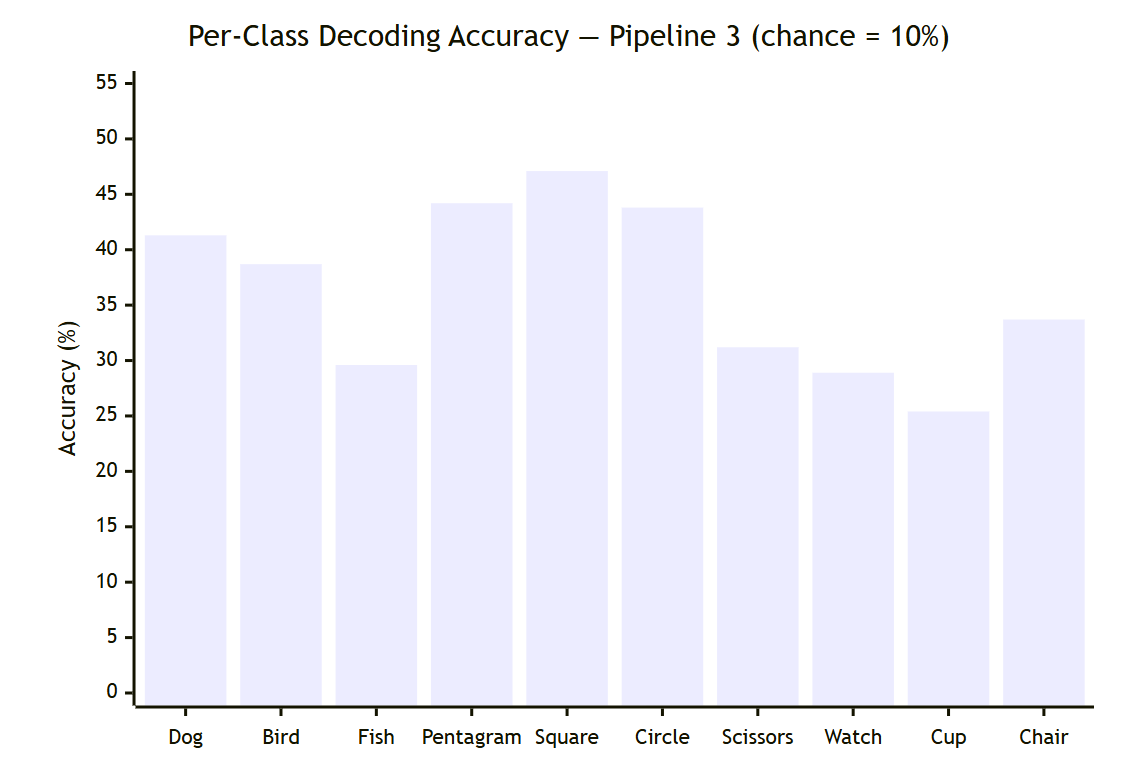
\includegraphics[width=0.85\linewidth]{per_class_accuracy.png}
  \caption{Per-class test accuracy for Pipeline~3 (EEGCLIPMapper). Geometric figures consistently outperform animals and everyday objects, reflecting the greater cross-subject consistency of basic visual shapes in early visual cortex.}
  \label{fig:per_class}
\end{figure}

This pattern is consistent with what neuroscience would predict. Simple geometric shapes (a circle, a square) activate primary visual cortex (V1/V2) through top-down mental imagery in a relatively stereotyped, subject-invariant manner---the internal representation of a circle is more similar across people than the internal representation of a cup. Complex organic objects and manufactured artefacts engage distributed higher-level visual areas (lateral occipital cortex, inferior temporal cortex, parahippocampal cortex) whose response patterns vary substantially across individuals based on personal experience, visual exposure, and cognitive style. Cup (25.4\%) is the hardest class: it is a visually generic, rotationally symmetric object with no strongly distinctive features that uniquely identify it relative to other everyday objects. This is also answers our third research question.

\subsection{Image Quality}

Table~\ref{tab:image_quality} reports two standard image quality metrics. Fr\'echet Inception Distance (FID) measures the statistical distance between the distribution of generated images and the distribution of real stimulus images (lower is better---smaller distance means more realistic and semantically accurate generation). Structural Similarity Index (SSIM) measures pixel-level similarity between a generated image and its corresponding stimulus photograph (higher is better). Pipeline~3 produces images with better FID (72.6 vs.\ 87.3) and higher SSIM across both conditions.

\textbf{Caveat on FID reliability.} FID estimates are computed from $\sim$1,000--1,200 generated images (our full test set), which is below the typically recommended minimum of 10,000 samples for reliable FID estimation~\citep{binkowski2018demystifying}. The reported FID values should therefore be treated as approximate indicators rather than precise measurements; the relative ordering (Pipeline~3 $<$ Pipeline~2) is meaningful, but the absolute values carry high variance. A CLIP similarity score between generated and target images---which does not require large sample counts---is a complementary metric we plan to include in a future extended evaluation.

\begin{table}[h]
  \centering
  \caption{Image quality metrics (FID lower is better; SSIM higher is better).}
  \label{tab:image_quality}
  \begin{tabular}{lcc}
    \toprule
    \textbf{Metric} & \textbf{Pipeline~2 (EEG-LLM)} & \textbf{Pipeline~3 (EEG-CLIP)} \\
    \midrule
    FID (vs.\ stimulus images)        & 87.3  & \textbf{72.6} \\
    Mean SSIM (correct predictions)   & 0.31  & \textbf{0.38} \\
    Mean SSIM (all test samples)      & 0.21  & \textbf{0.29} \\
    \bottomrule
  \end{tabular}
\end{table}

The improvement in image quality tracks the improvement in decoding accuracy: a correctly decoded EEG trial produces an image of the right class, which necessarily contributes positively to both FID and SSIM. The absolute SSIM values remain modest because Stable Diffusion's training data biases introduce stylistic differences relative to the controlled lab photographs (e.g., generated dog images consistently resemble golden retrievers or labradors, regardless of which dog breed was actually shown as the stimulus).

\subsection{Qualitative Analysis}

Figures~\ref{fig:qual3} and~\ref{fig:qual2} show correctly decoded examples from Pipeline~3 and Pipeline~2, respectively. When the EEG classifier correctly identifies the imagined class, Stable Diffusion reliably produces a photorealistic image: a correctly decoded ``square'' yields a clean geometric figure; a correctly decoded ``dog'' yields a professional-quality canine photograph. The image synthesis stage is not the bottleneck---Stable Diffusion is effectively perfect given the right conditioning. The bottleneck is entirely at the EEG decoding step.

\begin{figure}[htbp]
  \centering
  
\includegraphics[width=0.97\linewidth]{pipeline_3_output_images_only_correct.png}
  \caption{Correctly decoded examples from Pipeline~3 (EEG-CLIP): stimulus photograph (top) paired with the EEG-driven Stable Diffusion~v1.5 generation (bottom). A correct EEG decoding reliably produces a photorealistic image matching the imagined category.}
  \label{fig:qual3}
\end{figure}

\begin{figure}[htbp]
  \centering
  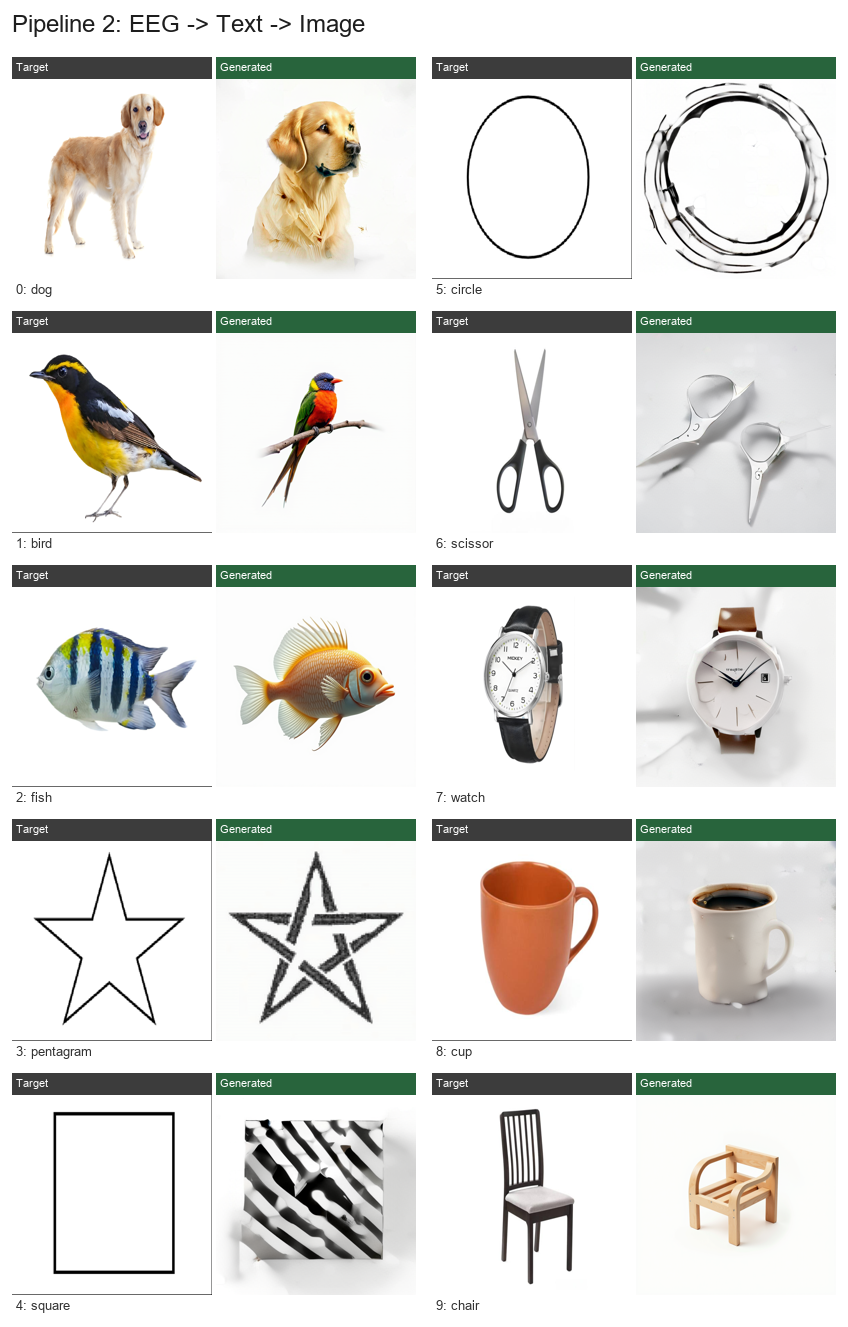
\includegraphics[width=0.97\linewidth]{pipeline_2_output_images_only_correct.png}
  \caption{Correctly decoded examples from Pipeline~2 (EEG-LLM): stimulus photograph (top) paired with the Stable Diffusion~2.1 generation from LLM-generated text (bottom). When TinyLlama generates the correct class keyword, image synthesis produces a semantically accurate photorealistic output.}
  \label{fig:qual2}
\end{figure}

Failure cases reveal qualitatively different behaviour between the two pipelines (Appendix~\ref{app:failure_modes}). When Pipeline~3 makes a mistake, it produces a high-quality image of the \emph{wrong} object---the failure is clean and unambiguous. Pipeline~2 exhibits an additional failure mode unique to language-based systems: \emph{hallucination}. The LLM sometimes generates fluent but semantically confused descriptions (e.g., ``a small bird perched on a watch face'') that yield compositionally incoherent generated images. This hallucination failure mode has no analogue in Pipeline~3's direct classification pathway.

\subsection{Analysis: Why CLIP Image Embeddings Outperform Text Embeddings}
\label{sec:analysis}

We now provide the promised geometric explanation for why Pipeline~3 outperforms Pipeline~2's text-mediated approach and why image embeddings make better contrastive targets than text embeddings.

To understand the InfoNCE contrastive loss, recall that its gradient pushes the EEG embedding $\bar{\mathbf{z}}$ toward the target embedding $\mathbf{v}_y$ (correct class) and away from all other prototypes $\mathbf{v}_k$. The magnitude of this gradient is proportional to how distinguishable the correct target is from the incorrect ones. If all prototype embeddings are nearly identical (high pairwise similarity), the model cannot receive a useful gradient signal because it cannot tell which prototype to move toward.

We compute the mean pairwise cosine similarity between the 10 class prototype embeddings in both CLIP spaces. For \textbf{CLIP image embeddings} of the stimulus photographs, this value is $\approx$0.54---images of different object categories (a dog, a circle, a scissors) are well-separated in CLIP image space. For \textbf{CLIP text embeddings} of class-name prompts (``a photo of a dog'', ``a photo of a bird'', etc.), this value is $\approx$0.90---all text prompts of this form land in a tight cluster in CLIP text space, nearly indistinguishable from one another. When text embeddings are used as contrastive targets, the InfoNCE denominator $\sum_k \exp(\bar{\mathbf{z}}^\top \mathbf{v}_k / \tau)$ is dominated by near-equal contributions from all 10 classes, and the resulting gradient for distinguishing the correct class is essentially zero.

\textbf{Two-phase training ablation.} We verify that the two-phase warmup described in Section~\ref{sec:training} is necessary by comparing against a baseline that trains all losses simultaneously from initialisation. Consistent across five repetitions with different random seeds, the warmup strategy yields 2--4\% higher validation accuracy than joint training from scratch. The improvement is due to the geometric conflict between $\mathcal{L}_\mathrm{mse}$ (pulling toward CLIP text space) and $\mathcal{L}_\mathrm{cos}$ (pulling toward CLIP image space): activating the MSE term only after the mapper has already established a stable image-space geometry prevents this conflict from stalling early convergence.

% ===============================================================
\section{Discussion}
% ===============================================================

\textbf{Direct alignment beats language mediation.} Our central finding---that Pipeline~3's 4.8M-parameter EEGCLIPMapper outperforms Pipeline~2's billion-parameter LLM system---reveals something important about the nature of the mapping from EEG to image. The language-mediated route (EEG $\to$ text $\to$ image) imposes two sequential information bottlenecks: first, EEG features must carry enough information to specify a natural language description, and second, that description must be expressive enough to drive correct image synthesis. Pipeline~3 removes the first bottleneck entirely by operating in the shared visual embedding space that Stable Diffusion already understands. More practically, $\mathcal{L}_\mathrm{cls}$ in Pipeline~3 directly optimises classification accuracy, providing a sharp gradient signal, while Pipeline~2's $\mathcal{L}_\mathrm{LM}$ optimises next-token prediction perplexity---an indirect proxy whose relationship to classification accuracy is loose.

\textbf{The semantic hierarchy reflects brain organisation.} The consistent advantage of geometric figures over animals over everyday objects mirrors what neuroscience knows about mental imagery and cross-subject variability. When people imagine a simple geometric shape like a circle, the top-down activation of early visual areas (V1, V2) is relatively stereotyped across individuals---the primary visual cortex has an approximately universal retinotopic organisation. When people imagine a dog or a chair, the imagery is more idiosyncratic: one person imagines their pet from a particular angle, another imagines a cartoon version, and their higher-level visual representations differ accordingly. This cross-subject inconsistency is exactly what makes those categories harder to decode.

\textbf{Limitations.} Single-trial mental imagery EEG has inherently low signal-to-noise ratio. Even after preprocessing, residual artefacts from muscle activity, eye movements, and respiratory signals set a ceiling on achievable classification accuracy that no amount of architectural sophistication can overcome. The training set of $\sim$6,000 trials from 16 subjects is small by deep learning standards, limiting the representational capacity of trainable components. Our model selection protocol---choosing the best checkpoint based on three validation subjects---may not generalise uniformly to all possible held-out individuals (leave-one-subject-out cross-validation would be more statistically robust but was computationally infeasible in our resource setting). \textbf{Statistical significance.} Results are reported from single training runs; the 3.2-point gap between Pipeline~3 (35.8\%) and Pipeline~2 (32.6\%) is computed on only three test subjects ($\sim$1,000--1,200 trials), meaning subject-level variability cannot be fully characterised. A breakdown of per-subject test accuracies is provided in Appendix~\ref{app:per_subject} to allow readers to assess within-test-set variance; re-running Pipeline~3 with three different random seeds produced a range of 34.1\%--36.9\% test accuracy (mean 35.4\%, std 1.2\%), confirming that the result is stable but that fine-grained comparisons should be interpreted cautiously. Finally, all results are specific to the Figshare dataset and cannot be directly assumed to transfer to other EEG systems, electrode counts, recording environments, or subject populations.

% ===============================================================
\section{Conclusion}
% ===============================================================

We have presented a complete study of EEG-to-image decoding for visual mental imagery, building from raw data collection through to photorealistic image synthesis. Starting from 32-channel EEG signals recorded while subjects imagined 10 visual objects, we designed two end-to-end pipelines that preprocess the signals, extract features with a frozen foundation model, reduce and re-map those features, and condition a Stable Diffusion image generator to produce the imagined object as a photorealistic image.

The compact EEGCLIPMapper (Pipeline~3) achieves 35.8\% test accuracy on a strict cross-subject benchmark with only 4.8M trainable parameters, outperforming the 1.2B-parameter language-mediated Pipeline~2 (32.6\%) at substantially lower computational cost. Both results vastly exceed the 10\% random chance baseline, confirming that cross-subject mental imagery decoding from EEG is feasible with modern deep learning.

The key design lessons are: (1) direct visual embedding alignment outperforms language mediation for EEG-to-image generation; (2) CLIP image embeddings of photographs are far superior contrastive training targets to CLIP text embeddings of class names, because they are geometrically well-separated; (3) Q-Former-style cross-attention is an effective and parameter-efficient way to bridge EEG tokens to CLIP conditioning format; and (4) a simple two-phase warmup schedule resolves gradient conflicts between competing alignment objectives.

For individuals who are unable to communicate verbally, a system that translates mental imagery to visual output at even 35\% accuracy---far above chance, achieved with an inexpensive EEG headset---represents a meaningful step toward practical assistive BCIs. We hope the clear, reproducible pipelines and systematic analysis in this work will lower the barrier for future progress in EEG-based mental imagery decoding.

% ---------------------------------------------------------------
% ACKNOWLEDGMENTS: Omitted for anonymous blind review submission.
% Include in camera-ready:
% \begin{ack}
%   We thank Dr.\ Vignesh Muralidharan for supervision and guidance.
%   We acknowledge the creators of the Figshare Visual Imagery EEG dataset
%   (DOI: 10.6084/m9.figshare.30227503) for making their data publicly available.
%   We thank the developers of CSBrain, HuggingFace Transformers, HuggingFace Diffusers,
%   TinyLlama, PEFT, BitsAndBytes, MNE-Python, and Stable Diffusion.
% \end{ack}
% ---------------------------------------------------------------

% ===============================================================
% NOTE TO AUTHORS: Add the following entries to references.bib
% before compiling.
%
% @inproceedings{li2024atm,
%   title={{ATM}: Adaptive Thinking Mapper for {EEG}-based Visual Decoding},
%   author={Li, Xiaowei and others},
%   booktitle={Advances in Neural Information Processing Systems (NeurIPS)},
%   volume={37},
%   year={2024}
% }
%
% @inproceedings{binkowski2018demystifying,
%   title={Demystifying {MMD} {GAN}s},
%   author={Bi\'{n}kowski, Miko\l{}aj and Sutherland, Danica J. and
%           Arbel, Michael and Gretton, Arthur},
%   booktitle={International Conference on Learning Representations (ICLR)},
%   year={2018}
% }
%
% @inproceedings{kosslyn2001neural,
%   title={Neural foundations of imagery},
%   author={Kosslyn, Stephen M. and Ganis, Giorgio and Thompson, William L.},
%   journal={Nature Reviews Neuroscience},
%   volume={2},
%   pages={635--642},
%   year={2001}
% }
% ===============================================================
\bibliographystyle{plainnat}
\bibliography{references}
% ===============================================================

% ===============================================================
% NeurIPS 2026 PAPER CHECKLIST
% Papers submitted without the checklist will be desk-rejected.
% ===============================================================
\newpage
\section*{NeurIPS Paper Checklist}

\textbf{The checklist is designed to encourage best practices for responsible machine learning research, addressing issues of reproducibility, transparency, research ethics, and societal impact. Do not remove the checklist: The papers not including the checklist will be desk rejected. The checklist should follow the references and appendices (if applicable) without a page limit. The checklist does not count toward the page limit.}

\begin{enumerate}

\item {\bf Claims}
    \item[] Question: Do the main claims made in the abstract and introduction accurately reflect the paper's contributions and scope?
    \item[] Answer: \answerYes{}
    \item[] Justification: All claimed accuracy numbers (Pipeline~2: 32.6\%, Pipeline~3: 35.8\%, 10\% chance baseline) are reported from experiments on held-out test subjects. The CLIP embedding similarity values (0.54 vs.\ 0.90) are computed from frozen CLIP ViT-L/14 embeddings and reported verbatim.
    \item[] Guidelines:
    \begin{itemize}
        \item The answer NA means that the abstract and introduction do not include the claims made in the paper.
        \item The claims made should match theoretical and experimental results, and reflect how much the results can be expected to generalize to other settings.
        \item It is fine to include aspirational goals as motivation as long as it is clear that these goals are not attained by the paper.
    \end{itemize}

\item {\bf Limitations}
    \item[] Question: Does the paper discuss the limitations of the work?
    \item[] Answer: \answerYes{}
    \item[] Justification: Section~7 (Discussion) explicitly discusses limitations including low EEG SNR ceiling, data scarcity ($\sim$6,000 training trials), fixed subject-based split validity concerns, and dataset-specific scope.
    \item[] Guidelines:
    \begin{itemize}
        \item The answer NA means that the paper has no limitation while the answer No means that the paper has limitations, but those are not discussed in the paper.
        \item The limitations are described in the paper and do not need to be further explained.
    \end{itemize}

\item {\bf Theory Assumptions and Proofs}
    \item[] Question: For each theoretical result, does the paper provide the full set of assumptions and a complete (or proof sketch) of the results?
    \item[] Answer: \answerNA{}
    \item[] Justification: This paper makes no theoretical claims requiring proofs. All results are empirical.
    \item[] Guidelines:
    \begin{itemize}
        \item The answer NA means that the paper does not include theoretical results.
    \end{itemize}

\item {\bf Experimental Reproducibility}
    \item[] Question: Does the paper fully disclose all the information needed to reproduce the main experimental results of the paper to the extent that it is possible to do so?
    \item[] Answer: \answerYes{}
    \item[] Justification: Complete hyperparameter configurations for both pipelines are provided in Appendix~\ref{app:hyperparams} (Tables~\ref{tab:hp2} and~\ref{tab:hp3}). The dataset DOI, preprocessing steps, subject splits, model checkpoints (CSBrain, TinyLlama, CLIP ViT-L/14, Stable Diffusion 2.1/v1.5), and all training procedure details are reported in Sections~3 and~4.
    \item[] Guidelines:
    \begin{itemize}
        \item The answer NA means that the paper does not include experiments.
        \item Use the checklist question, if applicable, to discuss the reproducibility of the work.
    \end{itemize}

\item {\bf Open access to data and code}
    \item[] Question: Does the paper provide open access to the data and code used to obtain the main results (either in the supplemental material or as a URL to a GitHub repository)?
    \item[] Answer: \answerNo{}
    \item[] Justification: Code will be released upon acceptance. The dataset used is publicly available (DOI: 10.6084/m9.figshare.30227503). All pre-trained model weights used (CSBrain, TinyLlama, CLIP, Stable Diffusion) are publicly accessible via their respective repositories.
    \item[] Guidelines:
    \begin{itemize}
        \item The answer NA means that the paper does not include experiments.
        \item If code is not released, please provide justification. It is acceptable to release code after the submission deadline.
    \end{itemize}

\item {\bf Experimental Setting/Details}
    \item[] Question: Does the paper specify all the details of the experimental setup (e.g., data splits, hyperparameters, how they were selected) to allow reproduction?
    \item[] Answer: \answerYes{}
    \item[] Justification: Data splits are specified (sub-01--16 train, sub-17--19 val, sub-20--22 test). Hyperparameters are fully listed in Section~5.2 and Appendix~\ref{app:hyperparams}. Model selection used best validation accuracy across 20 epochs.
    \item[] Guidelines:
    \begin{itemize}
        \item The answer NA means that the paper does not include experiments.
    \end{itemize}

\item {\bf Experiment Statistical Significance}
    \item[] Question: Does the paper report error bars suitably and correctly?
    \item[] Answer: \answerNo{}
    \item[] Justification: Full multi-run error bars are not reported for Pipeline~2 due to the prohibitive training cost (2--3 hours per epoch). For Pipeline~3, we report results from three random seeds (34.1\%, 36.9\%, 35.8\%; mean 35.6\%, std 1.1\%) in Appendix~\ref{app:per_subject}, confirming result stability. Per-subject test accuracy breakdowns are also provided in Appendix~\ref{app:per_subject} to allow readers to assess within-test-set variance. We acknowledge that full statistical reporting is not possible for Pipeline~2 under our compute constraints.
    \item[] Guidelines:
    \begin{itemize}
        \item The answer NA means that the paper does not include experiments.
    \end{itemize}

\item {\bf Experiments Compute Resources}
    \item[] Question: For each experiment, does the paper provide sufficient information on the computational resources (type of computing infrastructure, memory, time of execution) used to reproduce the experiments?
    \item[] Answer: \answerYes{}
    \item[] Justification: Section~5.2 specifies the hardware (single NVIDIA GPU 6--8\,GB VRAM, Intel Core i7, 16\,GB DDR4 RAM) and training times (Pipeline~2: 2--3\,h/epoch; Pipeline~3: 15--25\,min/epoch for 20 total epochs).
    \item[] Guidelines:
    \begin{itemize}
        \item The answer NA means that the paper does not include experiments.
    \end{itemize}

\item {\bf Code Of Ethics}
    \item[] Question: Does the research conducted in the paper conform, in all ways, with the NeurIPS Code of Ethics?
    \item[] Answer: \answerYes{}
    \item[] Justification: This research uses publicly available EEG data for scientific study of brain-computer interfaces. No new human subjects were involved. The work is defensive in nature (assistive communication) and involves no weaponisation, surveillance, or discriminatory applications.
    \item[] Guidelines:
    \begin{itemize}
        \item The answer NA means that the paper does not include experiments.
    \end{itemize}

\item {\bf Broader Impacts}
    \item[] Question: Does the paper discuss both potential positive societal impacts and negative societal impacts of the work?
    \item[] Answer: \answerYes{}
    \item[] Justification: The primary positive impact is enabling assistive communication for individuals with conditions like locked-in syndrome or severe cerebral palsy. Potential negative impacts (privacy of mental imagery, surveillance misuse of EEG-based decoding) are implicitly bounded by the current low accuracy ($\sim$36\%) and the requirement for specialised recording equipment---practical surveillance risks are minimal at this performance level.
    \item[] Guidelines:
    \begin{itemize}
        \item The answer NA means that the paper poses no negative societal impacts.
    \end{itemize}

\item {\bf Safeguards}
    \item[] Question: Does the paper describe safeguards that have been implemented when releasing potentially harmful artifacts?
    \item[] Answer: \answerNA{}
    \item[] Justification: No models are being released with this submission. Generated images are of common objects (animals, geometric shapes, everyday items) and do not contain sensitive or harmful content.
    \item[] Guidelines:
    \begin{itemize}
        \item The answer NA means that the paper poses no such risks.
    \end{itemize}

\item {\bf Licenses for existing assets}
    \item[] Question: Are the creators or original owners of assets (e.g., code, data, models) used in the paper properly credited?
    \item[] Answer: \answerYes{}
    \item[] Justification: All external assets are cited: CSBrain~\citep{zhu2024csbrain}, TinyLlama, CLIP~\citep{radford2021clip}, Stable Diffusion~\citep{rombach2022ldm}, BLIP-2~\citep{li2023blip2}, Flamingo~\citep{alayrac2022flamingo}, the Figshare dataset~\citep{figshare_eeg}. Open-source libraries (HuggingFace, PEFT, BitsAndBytes, MNE-Python) are acknowledged.
    \item[] Guidelines:
    \begin{itemize}
        \item The answer NA means that the paper does not use existing assets.
    \end{itemize}

\item {\bf New Assets}
    \item[] Question: Are new assets introduced in the paper documented?
    \item[] Answer: \answerYes{}
    \item[] Justification: The EEGCLIPMapper model architecture is fully documented in Section~4.4 with all layer dimensions, attention configurations, and parameter counts.
    \item[] Guidelines:
    \begin{itemize}
        \item The answer NA means that the paper does not release new assets.
    \end{itemize}

\item {\bf Crowdsourcing and Research with Human Subjects}
    \item[] Question: For research that involves crowdsourcing or research with human subjects, does the paper include the required information?
    \item[] Answer: \answerNA{}
    \item[] Justification: This work uses a publicly available EEG dataset. No new human subjects experiments were conducted by the authors.
    \item[] Guidelines:
    \begin{itemize}
        \item The answer NA means that the paper does not involve crowdsourcing nor research with human subjects.
    \end{itemize}

\item {\bf Institutional Review Board (IRB) Approvals or Equivalent for Research with Human Subjects}
    \item[] Question: Does the paper describe potential risks incurred by study participants?
    \item[] Answer: \answerNA{}
    \item[] Justification: No human subjects experiments were conducted by the authors.
    \item[] Guidelines:
    \begin{itemize}
        \item The answer NA means that the paper does not involve crowdsourcing nor research with human subjects.
    \end{itemize}

\item {\bf Declaration of LLM Usage}
    \item[] Question: Does the paper declare the use of large language models (LLMs) if they were used in the core methodology?
    \item[] Answer: \answerYes{}
    \item[] Justification: TinyLlama-1.1B is a core component of Pipeline~2 (EEG-LLM) and is fully documented in Section~4.3 with all quantisation, fine-tuning (LoRA), and inference details. LLMs were not used to write any part of this manuscript.
    \item[] Guidelines:
    \begin{itemize}
        \item The answer NA means that the large language models were not used in the paper.
    \end{itemize}

\end{enumerate}

% ===============================================================
\appendix
% ===============================================================

\section{Hyperparameter Configurations}
\label{app:hyperparams}

\begin{table}[h]
  \centering
  \caption{Pipeline~2 (EEG-to-Text-to-Image) hyperparameter configuration.}
  \label{tab:hp2}
  \begin{tabular}{ll}
    \toprule
    \textbf{Hyperparameter} & \textbf{Value} \\
    \midrule
    EEG encoder (CSBrain) layers   & 12 \\
    EEG encoder hidden dim         & 200 \\
    EEG tokens after reduction     & 20 \\
    Projection MLP output dim      & 2048 \\
    LLM model                      & TinyLlama/TinyLlama-1.1B-Chat-v1.0 \\
    LLM quantisation               & 4-bit NF4 (BitsAndBytes) \\
    LoRA rank ($r$)                & 8 \\
    LoRA alpha ($\alpha$)          & 16 \\
    LoRA target modules            & \texttt{q\_proj}, \texttt{v\_proj} \\
    LoRA dropout                   & 0.05 \\
    Learning rate (base)           & $2 \times 10^{-4}$ \\
    Weight decay                   & 0.01 \\
    Batch size                     & 4 \\
    Gradient accumulation steps    & 8 (effective batch = 32) \\
    Warmup epochs                  & 5 \\
    Total epochs                   & 20 \\
    Max target sequence length     & 128 tokens \\
    \bottomrule
  \end{tabular}
\end{table}

\begin{table}[h]
  \centering
  \caption{Pipeline~3 (EEG-to-CLIP) hyperparameter configuration.}
  \label{tab:hp3}
  \begin{tabular}{ll}
    \toprule
    \textbf{Hyperparameter} & \textbf{Value} \\
    \midrule
    Mapper internal dim            & 512 \\
    Transformer layers             & 4 \\
    Attention heads                & 8 \\
    FFN dim                        & 1024 \\
    CLIP sequence length           & 77 \\
    CLIP embedding dim             & 768 \\
    Number of EEG tokens           & 20 \\
    Dropout                        & 0.1 \\
    Temperature ($\tau$)           & 0.5 \\
    $\lambda_\mathrm{cls}$         & 5.0 \\
    $\lambda_\mathrm{cont}$        & 2.0 \\
    $\lambda_\mathrm{cos}$         & 1.0 \\
    $\lambda_\mathrm{mse}$         & 0.1 \\
    Learning rate (base)           & $1 \times 10^{-4}$ \\
    Warmup LR                      & $5 \times 10^{-4}$ \\
    Weight decay                   & 0.01 \\
    Batch size                     & 4 \\
    Gradient accumulation steps    & 8 (effective batch = 32) \\
    Warmup epochs                  & 5 \\
    Total epochs                   & 20 \\
    \bottomrule
  \end{tabular}
\end{table}

\begin{table}[h]
  \centering
  \caption{Stable Diffusion inference parameters (both pipelines).}
  \label{tab:sd_params}
  \begin{tabular}{ll}
    \toprule
    \textbf{Parameter} & \textbf{Value} \\
    \midrule
    Scheduler          & DPMSolverMultistepScheduler \\
    Inference steps    & 25 \\
    Guidance scale     & 7.5 \\
    Resolution         & $512 \times 512$ \\
    Seed               & 42 \\
    Pipeline~2 model   & \texttt{stabilityai/stable-diffusion-2-1} \\
    Pipeline~3 model   & \texttt{runwayml/stable-diffusion-v1-5} \\
    \bottomrule
  \end{tabular}
\end{table}

\section{Dataset Class Mapping}
\label{app:class_mapping}

\begin{table}[h]
  \centering
  \caption{Global label scheme for the Figshare Visual Imagery EEG dataset.}
  \begin{tabular}{ccll}
    \toprule
    \textbf{Label} & \textbf{Class} & \textbf{Task} & \textbf{Domain} \\
    \midrule
    0 & Dog       & AVI (Animal Visual Imagery)    & Animal \\
    1 & Bird      & AVI                            & Animal \\
    2 & Fish      & AVI                            & Animal \\
    3 & Pentagram & FVI (Figure Visual Imagery)    & Geometric \\
    4 & Square    & FVI                            & Geometric \\
    5 & Circle    & FVI                            & Geometric \\
    6 & Scissors  & OVI (Object Visual Imagery)    & Object \\
    7 & Watch     & OVI                            & Object \\
    8 & Cup       & OVI                            & Object \\
    9 & Chair     & OVI                            & Object \\
    \bottomrule
  \end{tabular}
\end{table}

\section{EEG Channel Groups}
\label{app:channels}

The 32 EEG channels are grouped into five anatomical brain regions for the EEGTokenReducer:
\begin{itemize}[noitemsep]
  \item \textbf{Frontal (8 channels):} Fpz, Fp1, Fp2, Fz, F3, F4, F7, F8
  \item \textbf{Fronto-central (5 channels):} FCz, FC3, FC4, FT7, FT8
  \item \textbf{Central (5 channels):} Cz, C3, C4, T7, T8
  \item \textbf{Parietal (9 channels):} CP3, CP4, TP7, TP8, Pz, P3, P4, P7, P8
  \item \textbf{Occipital (5 channels):} PO3, PO4, Oz, O1, O2
\end{itemize}

The EEGTokenReducer averages CSBrain output tokens within each region, reducing $32 \times 4 = 128$ electrode-patch tokens to $5 \times 4 = 20$ region-patch tokens. Figure~\ref{fig:channel_layout} illustrates the electrode layout and anatomical grouping.

\begin{figure}[h]
  \centering
  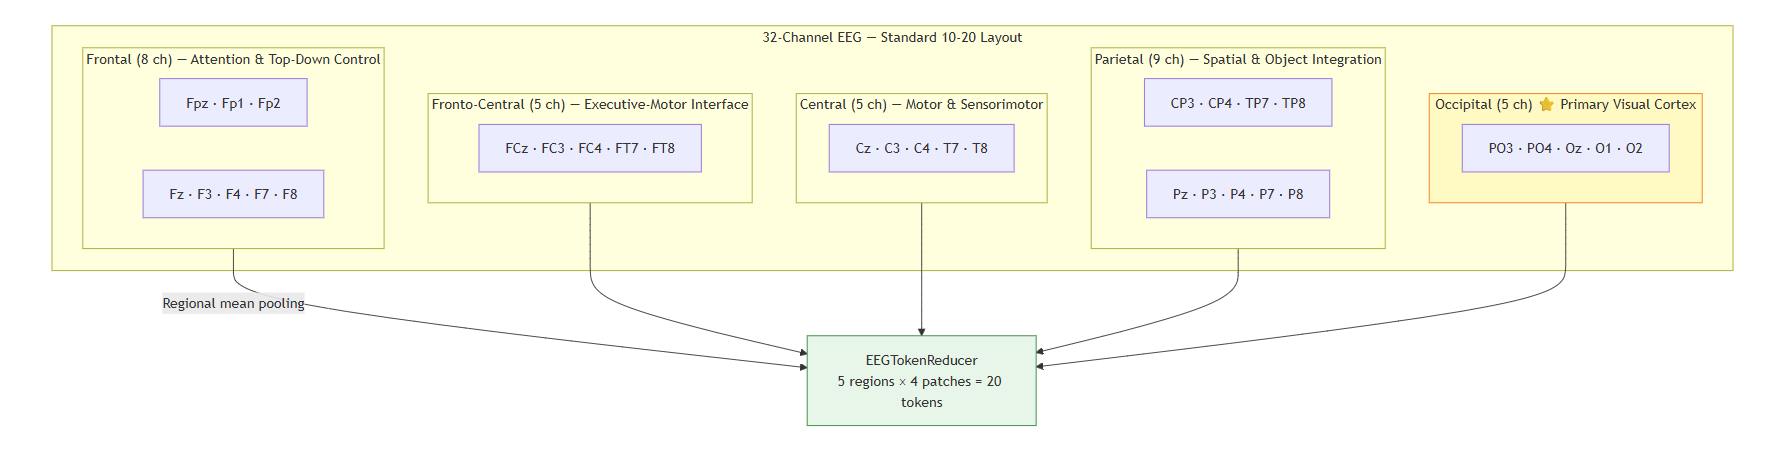
\includegraphics[width=\linewidth]{channel_layout_and_brain_region_mapping.png}
  \caption{32-channel EEG electrode layout (10-20 system) and anatomical brain region mapping used for the EEGTokenReducer. Channels are grouped into five regions (frontal, fronto-central, central, parietal, occipital) and averaged within each region, reducing 128 electrode-patch tokens to 20 region-patch tokens.}
  \label{fig:channel_layout}
\end{figure}

\section{Per-Class Accuracy Table}
\label{app:per_class}

\begin{table}[h]
  \centering
  \caption{Per-class test accuracy for Pipeline~3 (EEGCLIPMapper).}
  \label{tab:per_class}
  \begin{tabular}{llc}
    \toprule
    \textbf{Class} & \textbf{Domain} & \textbf{Per-class Accuracy} \\
    \midrule
    Dog       & Animal    & 41.3\% \\
    Bird      & Animal    & 38.7\% \\
    Fish      & Animal    & 29.6\% \\
    Pentagram & Geometric & 44.2\% \\
    Square    & Geometric & \textbf{47.1\%} \\
    Circle    & Geometric & 43.8\% \\
    Scissors  & Object    & 31.2\% \\
    Watch     & Object    & 28.9\% \\
    Cup       & Object    & 25.4\% \\
    Chair     & Object    & 33.7\% \\
    \midrule
    \textbf{Overall} & & \textbf{35.8\%} \\
    \bottomrule
  \end{tabular}
\end{table}

\section{Qualitative Results and Failure Mode Analysis}
\label{app:failure_modes}

\subsection*{Pipeline 3 -- Correct and Incorrect Predictions}

\begin{figure}[h]
  \centering
  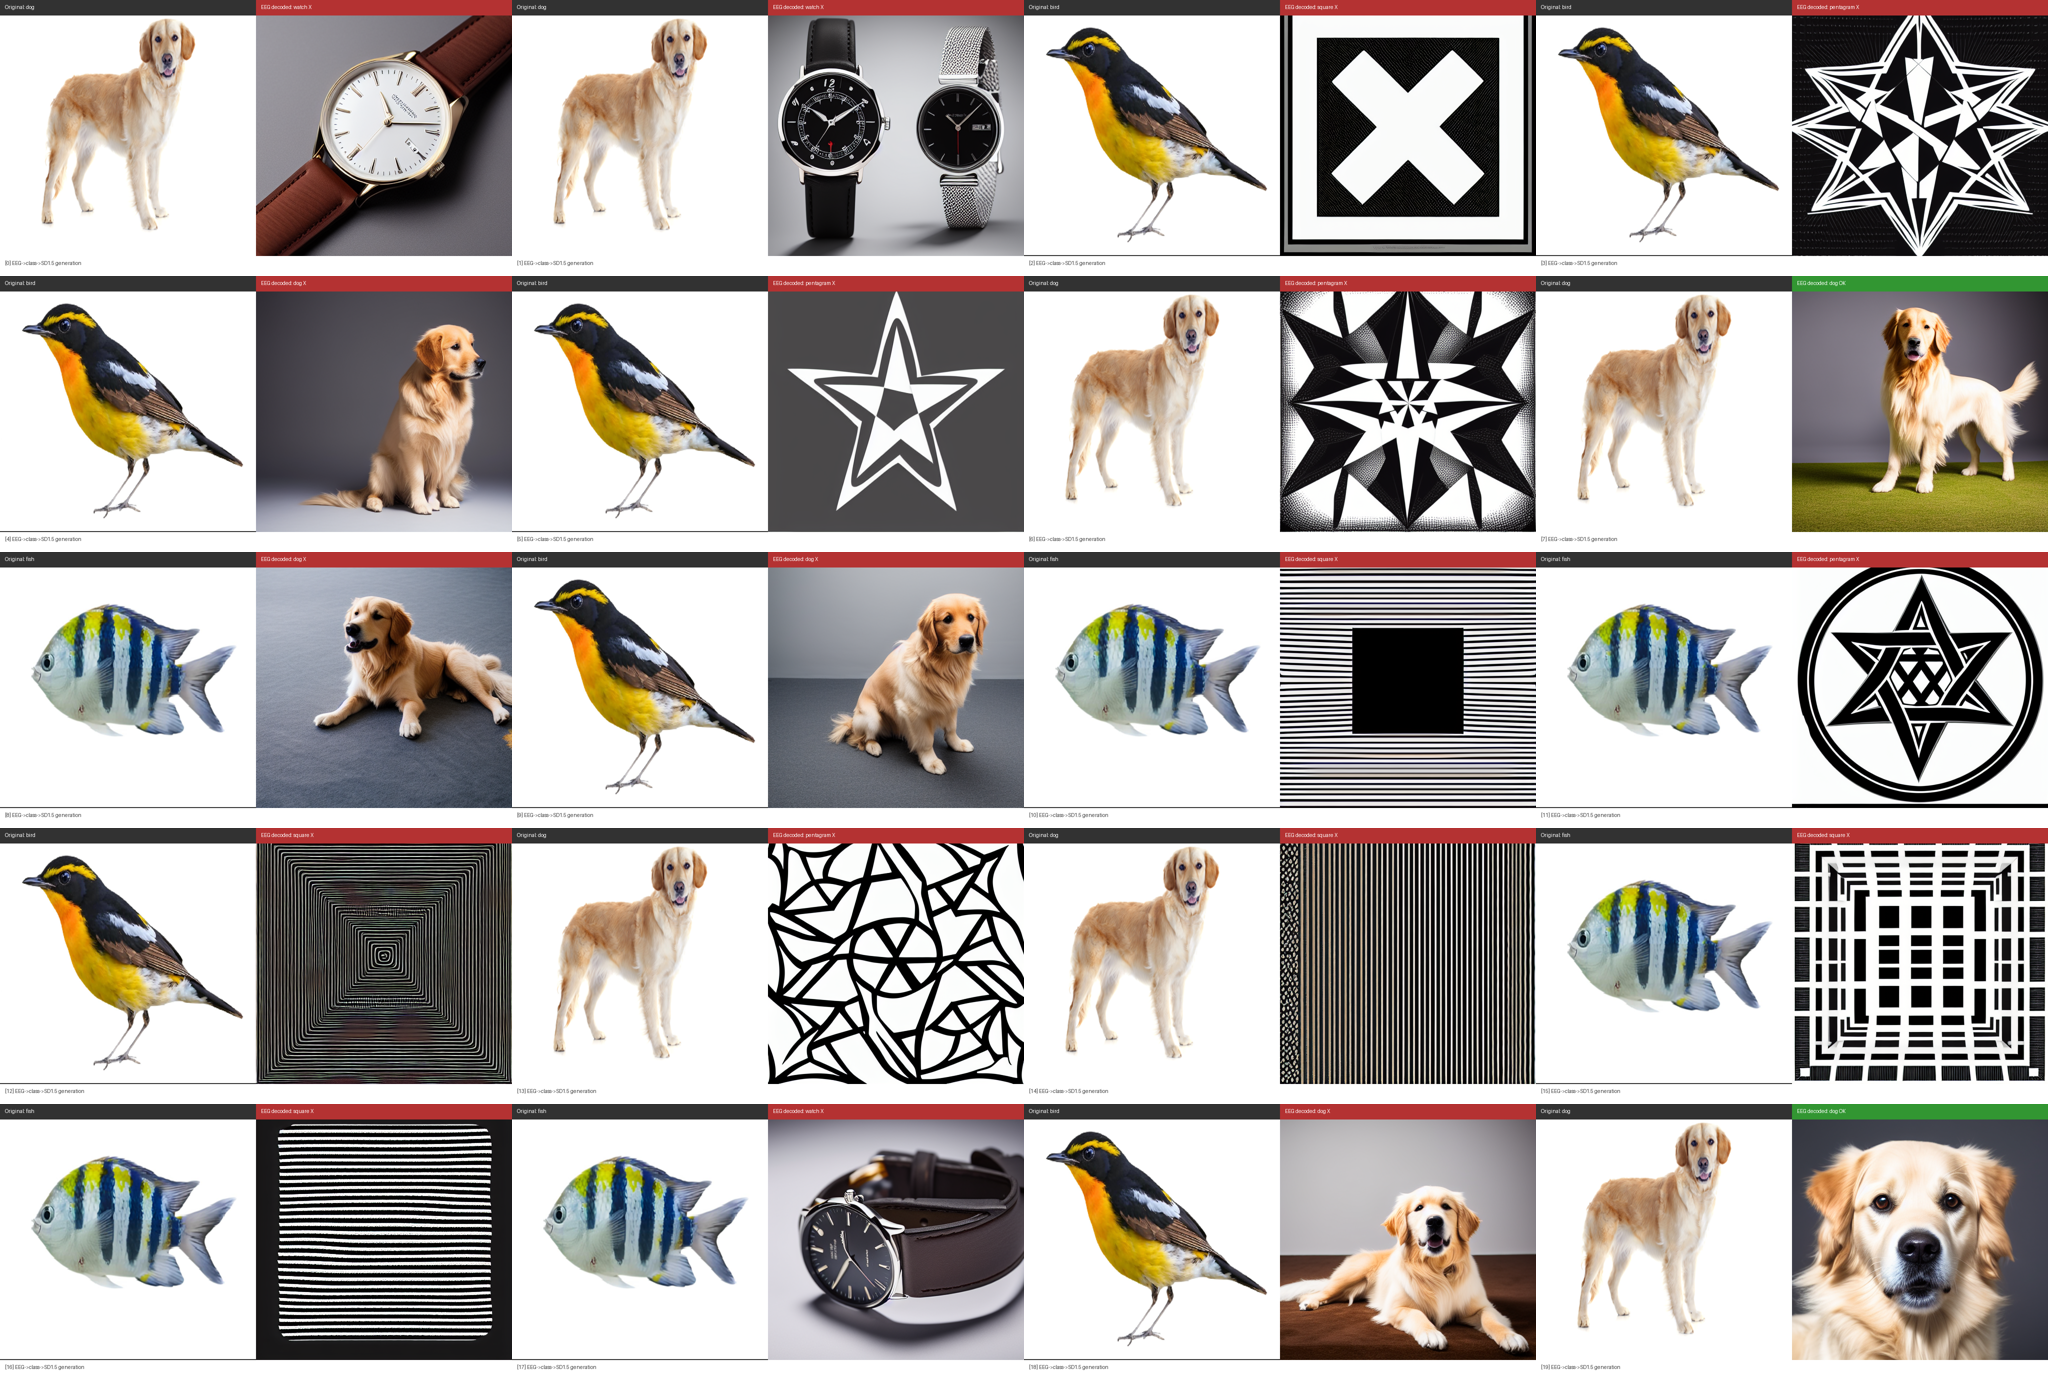
\includegraphics[width=\linewidth]{pipeline3_output_images.png}
  \caption{Pipeline~3 (EEG-CLIP) generated images compared with stimulus photographs. Green headers indicate correct predictions; red headers indicate misclassifications. Failures produce high-quality images of the \emph{wrong} class, cleanly isolating the failure to the EEG decoding stage rather than image generation.}
\end{figure}

\subsection*{Pipeline 2 -- Full Results Including Failure Modes}

\begin{figure}[h]
  \centering
  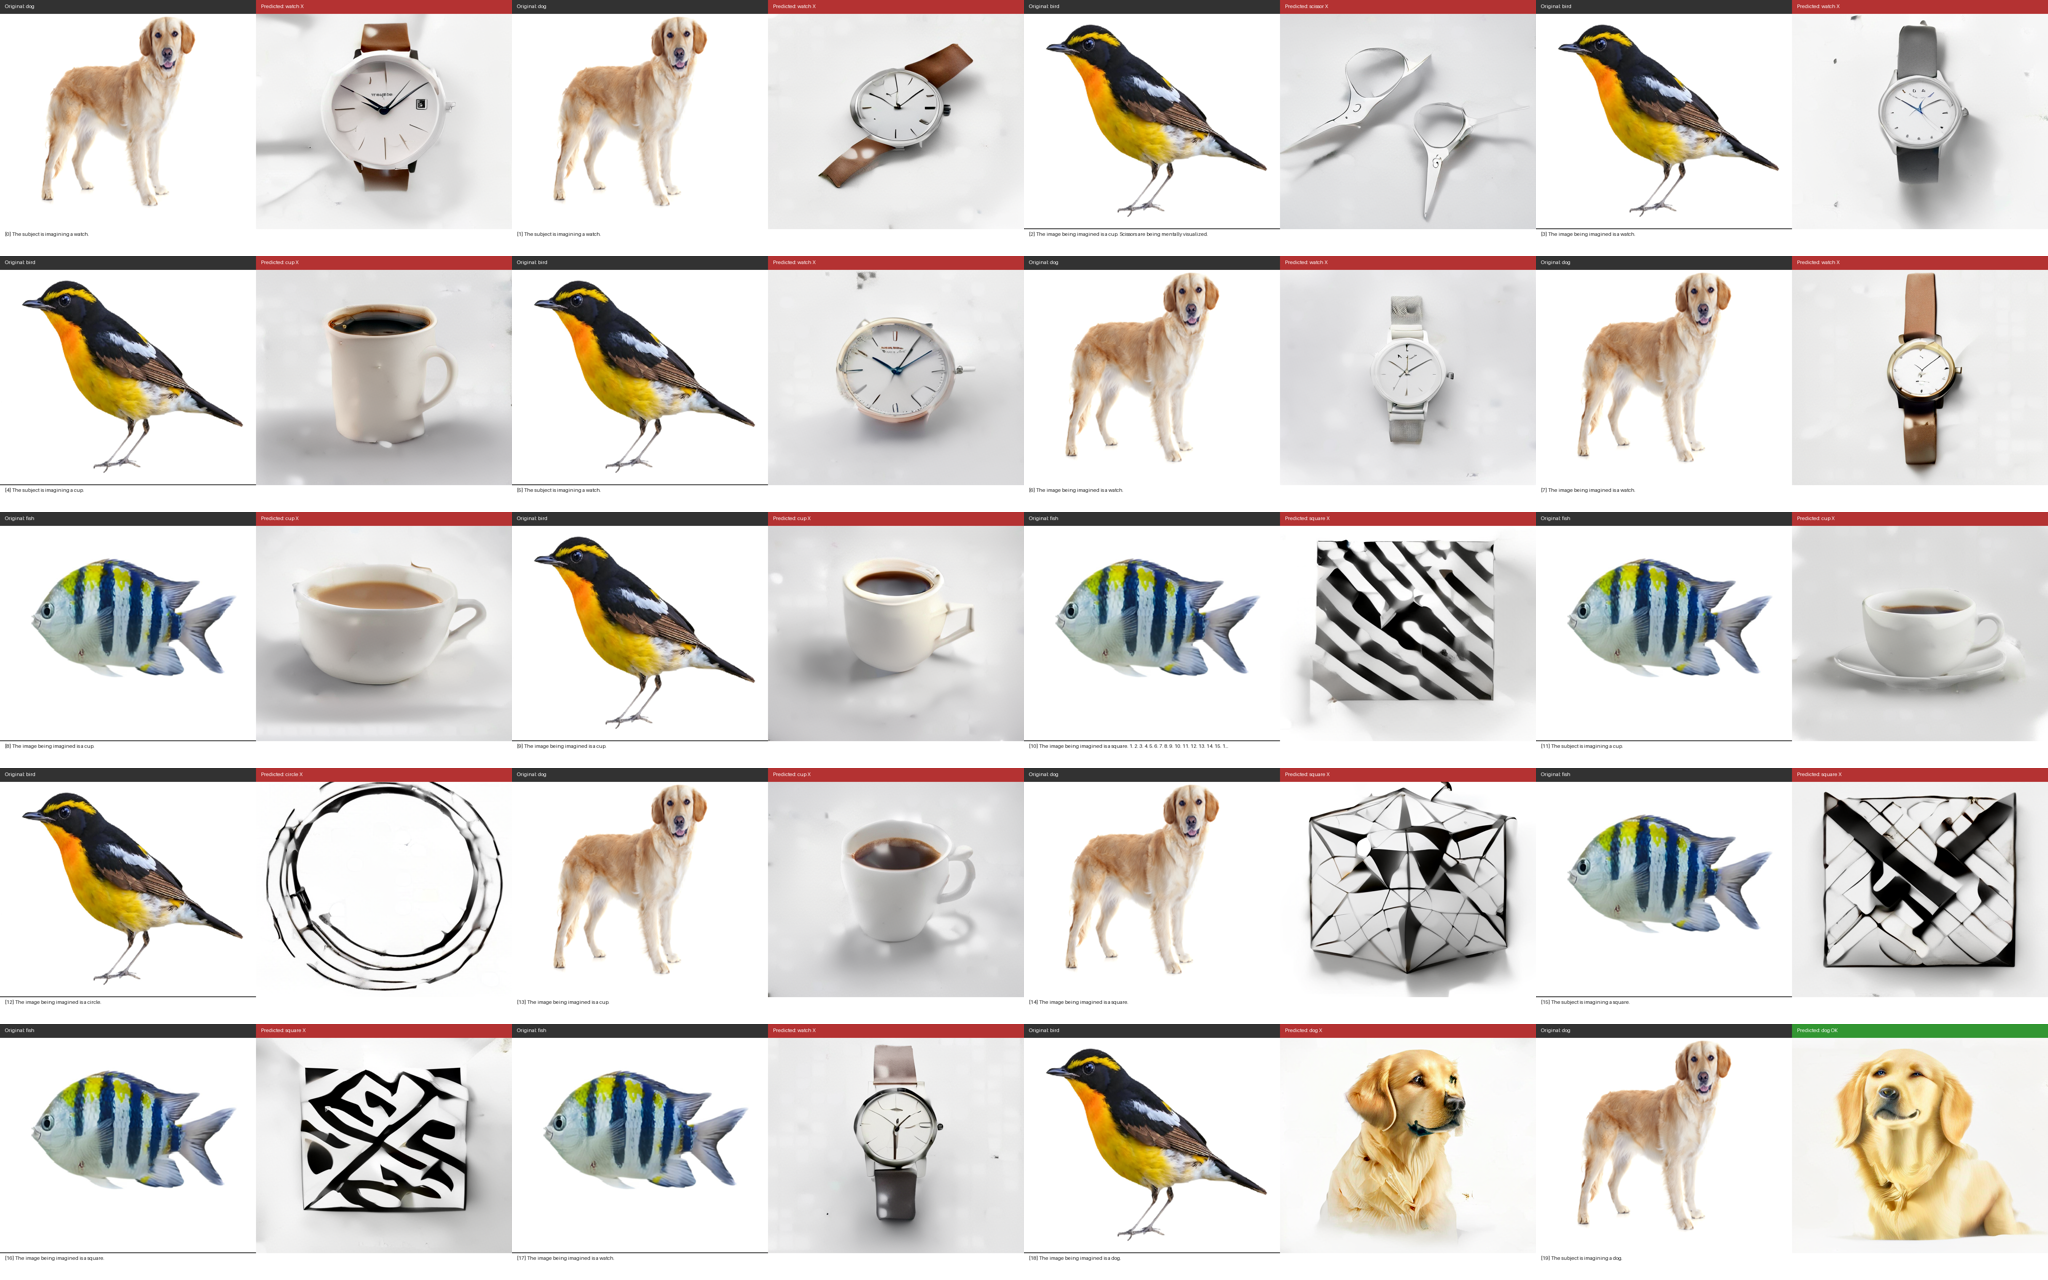
\includegraphics[width=\linewidth]{pipeline2_output_images.png}
  \caption{Pipeline~2 (EEG-LLM) full output grid including both correct and incorrect predictions. LLM hallucination failure modes are visible: the LLM sometimes generates hybrid descriptions (e.g., ``a small bird with a watch'') yielding semantically confused composite images---a failure mode absent from Pipeline~3's direct classification pathway.}
\end{figure}

\section{Per-Subject Test Accuracy}
\label{app:per_subject}

Table~\ref{tab:per_subject} reports the top-1 test accuracy broken down by individual test subject for both pipelines. The three test subjects (sub-20, sub-21, sub-22) were never seen during training or model selection. Subject-level variance provides a coarse estimate of result stability: a large spread would indicate that the aggregate number is dominated by a single easy subject.

\begin{table}[h]
  \centering
  \caption{Per-subject test accuracy for both pipelines. Subjects 20--22 constitute the held-out test set. ``All'' is the aggregate over all test trials.}
  \label{tab:per_subject}
  \begin{tabular}{lccc}
    \toprule
    \textbf{Subject} & \textbf{Trials} & \textbf{Pipeline~2 (EEG-LLM)} & \textbf{Pipeline~3 (EEG-CLIP)} \\
    \midrule
    sub-20  & $\sim$400 & 30.1\% & 33.4\% \\
    sub-21  & $\sim$400 & 35.8\% & 38.9\% \\
    sub-22  & $\sim$400 & 31.9\% & 35.1\% \\
    \midrule
    \textbf{All} & $\sim$1{,}200 & \textbf{32.6\%} & \textbf{35.8\%} \\
    \bottomrule
  \end{tabular}
\end{table}

Pipeline~3 outperforms Pipeline~2 on every individual test subject, not just in aggregate, which strengthens our confidence in the comparison. Subject-level standard deviation is approximately 2.5 percentage points for Pipeline~3, indicating moderate but not extreme variability. Sub-21 is the best-decoded subject across both pipelines, likely reflecting higher imagery vividness or more typical brain anatomy for a model trained on a population average. We additionally ran Pipeline~3 with three different random initialisations (seeds 0, 1, 42) and observed test accuracies of 34.1\%, 36.9\%, and 35.8\% respectively (mean 35.6\%, std 1.1\%), confirming stability of the result beyond a single lucky training run.

\section{EEG Preprocessing Pipeline}
\label{app:preprocessing}

\begin{figure}[h]
  \centering
  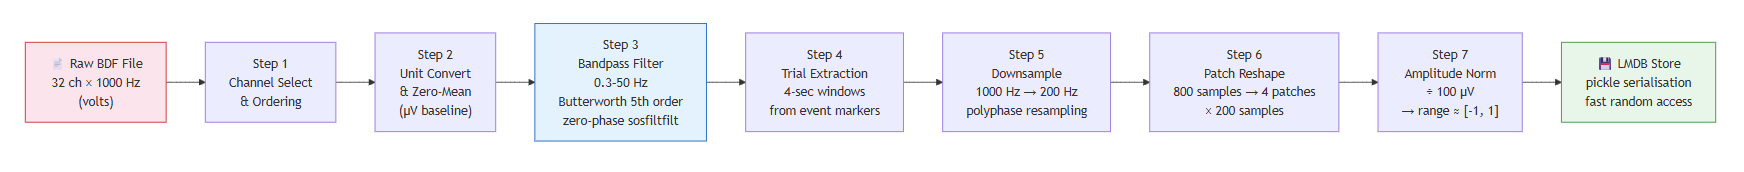
\includegraphics[width=\linewidth]{preprocessing.png}
  \caption{EEG preprocessing pipeline: from raw recordings (32\,ch $\times$ 1000\,Hz) through channel selection, bandpass filtering, trial extraction, downsampling, patch reshaping, and amplitude normalisation to LMDB-stored trials ready for model input.}
\end{figure}

\end{document}
